
% Outline: 28 Jan 2019
%   - 0. Summary (PAPPG guidlines) - 1p
%   - 1. Project Description - 10 pp
%   - 1.1 Intellectual Merit:
%       - 1.1.1 Background \& Motivation
%           - LSST cost NSF ~ \$1B
%               - LSST Science goals
%           - Can think of LSST as the next generation SDSS
%               - But it doesn't have spectroscopy!
%           - SDSS was an Imaging + Spectroscopy survey
%               - SDSS the most cited survey ever
%               - SDSS science milestones
%               - Spectroscopy was a key aspect for the success of SDSS
%                 (MPA-JHU)
%               - Public release of data also key
%           - What would it look like to perform SDSS-like spectroscopy
%             for the LSST imagine survey?
%               - Fraction of observed objects
%               - Cost
%               - currently an intractible problem
%                   - link to photonics development?
%               - Need new techniques (machine learning) to infer
%                 statistically accurate population characteristics with
%                 small training sets
%           - LSST Science themes
%           - Science enabled by LSST spectroscopy, lay groundwork for
%             later science discussion.
%
%       - 1.1.2 Research Community Priority
%           - Review Astro2010
%               - LSST
%           - Preview of or predictions for astro2020
%           - Big data initiatives:
%               - Moore-Sloan Data-Science Environments
%                   - Berkeley institute for data science, NYU, UW
%               - Using subsets of training data to understand a
%                 population
%                   - Hogg's AAS talk...
%
%           - Spectroscopy of LSST sources to get photozs provides key
%             advantages to Cosmology/Dark Energy
%           - Time domain astrophysics
%               - AGN, CVs, stars (astroseismology)
%
%       - 1.1.3 Astrophysics and Data Science Goals
%           - A Universe in transition
%               - Gravity to Dark Energy:
%                   - Precise cosmology with LSST and trained photozs
%               - Gas to stellar dominated: The Galactic Ecosystem at z~2
%                   - environment (Cooper)
%                   - absorption-line systems (Prochaska)
%                   - stellar populations (Shapely, Siana)
%                       - Bootstrap z~2 properties to higher redshift (z~7)
%               - Neutral to ionized gas: The heterogeneity of
%                 Reionization
%                   - environment and neutral fractions (Becker)
%                   - Ly continuum (photon budget) at z~5-7 (Siana)
%           - The Chemodynamical history of the Local Group
%               - Chemical tagging of GAIA spectra on the far side of
%                 the Milky Way (Yuan-Sen)
%                   - What's gained in 0.31-0.4 range (unavailable to
%                     PFS)
%               - MW/M31/M33 (Raja, Connie)
%               - Life cycle of stellar clusters
%           - Time Domain (Foley)
%
%       - 1.1.4 FOBOS
%           - How does FOBOS meet the science goals?
%           - Instrument description as of conceptual design
%           - Development from concept to final design
%               - Sketch of timeline
%           - Public survey design
%               - Key science programs
%               - AI-informed targeting system
%               - Robust DRP and DAP
%               - Public release schedule
%           - Longer-term strategy for public release of *any* FOBOS
%             data
%               - 18-month proprietary period for PI data
%               - Observatory queue for opportunistic use of "free"
%                 fibers
%
%       - 1.2 Broader Impacts
%           - Student Training
%           - ISEE, AKAMAI (Lisa Hunter)
%           - New UCSC Astrophysics major with Data Science emphasis
%               - New course, summer projects
%   
%   - 2. References (2-page max)
%
%   - 3. Biographical Sketches (2 pages each), required for PI, co-PIs,
%     and any additional senior personnel (see PAPPG)
%
%   - 4. Budget and Budget Justification: "For preliminary proposals
%     cost estimates may be preliminary estimates with the Basis of
%     Estimates (BoE) included. Copies of vendor quotations should not
%     be included in preliminary proposals. If the budget includes
%     contingency, that contingency should cover the 'known unknowns'
%     and be used to mitigate identified risks."
%
%   - 5. Facilities, Equipment, and Other Resources: "In order for NSF,
%     and its reviewers, to assess the scope of a proposed project, all
%     organizational resources necessary for, and available to a
%     project, must be described in this section of the proposal.
%     Proposers should describe only those resources that are directly
%     applicable. The description should be narrative in nature and must
%     not include any quantifiable financial information. Proposers
%     should include a description of the internal and external
%     resources (both physical and personnel) that are expected to be
%     available to the project.  Such information must be provided in
%     this section, in lieu of other parts of the proposal (e.g., Budget
%     Justification, Project Description)."
%
%   - 6. Supplementary Documents:
%           - A list of the major team members, their affiliations, and
%             their role in the project
%           - A list of Partner Organizations to be funded via
%             subawards, and the role of each in the project
%           - An outline of the Project Execution Plan (PEP) . See the
%             LFM/MFG. Greater detail will be required in invited full
%             proposals should that occur.
%
%         "No other items or appendices should be included. Information
%         pertaining to 'Results from Prior NSF Support', 'Current and
%         Pending Support', 'Data Management Plan', and 'Postdoctoral
%         Mentoring Plan' is not required for preliminary proposals and
%         should not be included. Preliminary proposals containing items
%         other than those required above will be returned without
%         review.


%\documentclass[11pt,letterpaper]{article}
\documentclass[oneside,11pt]{amsart}

%\usepackage{a4wide}
%\usepackage{epsfig}
%\usepackage{psfig}
\usepackage{graphicx}
\usepackage{natbib,latexsym,url,enumitem,pdfpages}
\usepackage{color}
\usepackage{wrapfig}

% Some fancy commenting
\definecolor{todo}{RGB}{200,0,0}
\newcommand{\comment}[2][todo]{{\color{#1}[[{\bf #2}]]}}

% Challenge counter
\newcounter{chalno}
\newcommand{\chal}[1]{\refstepcounter{chalno}\label{#1}}

% User commands
\makeatletter
\let\jnl@style=\rm
\def\ref@jnl#1{{\jnl@style#1}}

\def\ref@jnl#1{{\jnl@style#1}}% 
\newcommand\aj{\ref@jnl{AJ}}%        % Astronomical Journal 
\newcommand\araa{\ref@jnl{ARA\&A}}%  % Annual Review of Astron and Astrophys 
\newcommand\apj{\ref@jnl{ApJ}}%    % Astrophysical Journal ++
\newcommand\apjl{\ref@jnl{ApJL}}     % Astrophysical Journal, Letters 
\newcommand\apjs{\ref@jnl{ApJS}}%    % Astrophysical Journal, Supplement 
\newcommand\ao{\ref@jnl{ApOpt}}%   % Applied Optics ++
\newcommand\apss{\ref@jnl{Ap\&SS}}%  % Astrophysics and Space Science 
\newcommand\aap{\ref@jnl{A\&A}}%     % Astronomy and Astrophysics 
\newcommand\aapr{\ref@jnl{A\&A~Rv}}%  % Astronomy and Astrophysics Reviews 
\newcommand\aaps{\ref@jnl{A\&AS}}%    % Astronomy and Astrophysics, Supplement 
\newcommand\azh{\ref@jnl{AZh}}%       % Astronomicheskii Zhurnal 
\newcommand\baas{\ref@jnl{BAAS}}%     % Bulletin of the AAS 
\newcommand\icarus{\ref@jnl{Icarus}}% % Icarus
\newcommand\jrasc{\ref@jnl{JRASC}}%   % Journal of the RAS of Canada 
\newcommand\memras{\ref@jnl{MmRAS}}%  % Memoirs of the RAS 
\newcommand\mnras{\ref@jnl{MNRAS}}%   % Monthly Notices of the RAS 
\newcommand\pra{\ref@jnl{PhRvA}}% % Physical Review A: General Physics ++
\newcommand\prb{\ref@jnl{PhRvB}}% % Physical Review B: Solid State ++
\newcommand\prc{\ref@jnl{PhRvC}}% % Physical Review C ++
\newcommand\prd{\ref@jnl{PhRvD}}% % Physical Review D ++
\newcommand\pre{\ref@jnl{PhRvE}}% % Physical Review E ++
\newcommand\prl{\ref@jnl{PhRvL}}% % Physical Review Letters 
\newcommand\pasp{\ref@jnl{PASP}}%     % Publications of the ASP 
\newcommand\pasj{\ref@jnl{PASJ}}%     % Publications of the ASJ 
\newcommand\qjras{\ref@jnl{QJRAS}}%   % Quarterly Journal of the RAS 
\newcommand\skytel{\ref@jnl{S\&T}}%   % Sky and Telescope 
\newcommand\solphys{\ref@jnl{SoPh}}% % Solar Physics 
\newcommand\sovast{\ref@jnl{Soviet~Ast.}}% % Soviet Astronomy 
\newcommand\ssr{\ref@jnl{SSRv}}% % Space Science Reviews 
\newcommand\zap{\ref@jnl{ZA}}%       % Zeitschrift fuer Astrophysik 
\newcommand\nat{\ref@jnl{Nature}}%  % Nature 
\newcommand\iaucirc{\ref@jnl{IAUC}}% % IAU Cirulars 
\newcommand\aplett{\ref@jnl{Astrophys.~Lett.}}%  % Astrophysics Letters 
\newcommand\apspr{\ref@jnl{Astrophys.~Space~Phys.~Res.}}% % Astrophysics Space Physics Research 
\newcommand\bain{\ref@jnl{BAN}}% % Bulletin Astronomical Institute of the Netherlands 
\newcommand\fcp{\ref@jnl{FCPh}}%   % Fundamental Cosmic Physics 
\newcommand\gca{\ref@jnl{GeoCoA}}% % Geochimica Cosmochimica Acta 
\newcommand\grl{\ref@jnl{Geophys.~Res.~Lett.}}%  % Geophysics Research Letters 
\newcommand\jcp{\ref@jnl{JChPh}}%     % Journal of Chemical Physics 
\newcommand\jgr{\ref@jnl{J.~Geophys.~Res.}}%     % Journal of Geophysics Research 
\newcommand\jqsrt{\ref@jnl{JQSRT}}%   % Journal of Quantitiative Spectroscopy and Radiative Trasfer 
\newcommand\memsai{\ref@jnl{MmSAI}}% % Mem. Societa Astronomica Italiana 
\newcommand\nphysa{\ref@jnl{NuPhA}}%     % Nuclear Physics A 
\newcommand\physrep{\ref@jnl{PhR}}%       % Physics Reports 
\newcommand\physscr{\ref@jnl{PhyS}}%        % Physica Scripta 
\newcommand\planss{\ref@jnl{Planet.~Space~Sci.}}%  % Planetary Space Science 
\newcommand\procspie{\ref@jnl{Proc.~SPIE}}%      % Proceedings of the SPIE 

\newcommand\actaa{\ref@jnl{AcA}}%  % Acta Astronomica
\newcommand\caa{\ref@jnl{ChA\&A}}%  % Chinese Astronomy and Astrophysics
\newcommand\cjaa{\ref@jnl{ChJA\&A}}%  % Chinese Journal of Astronomy and Astrophysics
\newcommand\jcap{\ref@jnl{JCAP}}%  % Journal of Cosmology and Astroparticle Physics
\newcommand\na{\ref@jnl{NewA}}%  % New Astronomy
\newcommand\nar{\ref@jnl{NewAR}}%  % New Astronomy Review
\newcommand\pasa{\ref@jnl{PASA}}%  % Publications of the Astron. Soc. of Australia
\newcommand\rmxaa{\ref@jnl{RMxAA}}%  % Revista Mexicana de Astronomia y Astrofisica

%% added feb 9, 2016
\newcommand\maps{\ref@jnl{M\&PS}}% Meteoritics and Planetary Science
\newcommand\aas{\ref@jnl{AAS Meeting Abstracts}}% American Astronomical Society Meeting Abstracts
\newcommand\dps{\ref@jnl{AAS/DPS Meeting Abstracts}}% American Astronomical Society/Division for Planetary Sciences Meeting Abstracts



\let\astap=\aap 
\let\apjlett=\apjl 
\let\apjsupp=\apjs 
\let\applopt=\ao 



\DeclareRobustCommand{\gtrsim}{%
\mathrel{\hskip-.5em\begin{array}{c}>\\[-8pt]\sim\end{array}\hskip-.5em}}
\DeclareRobustCommand{\lesssim}{%
\mathrel{\hskip-.5em\begin{array}{c}<\\[-8pt]\sim\end{array}\hskip-.5em}}

\pretolerance=10000
\textwidth=6.4in
\textheight=8.95in
\voffset = 0.in
%\voffset = -0.3in  % For my printer
\topmargin=0.0in
\headheight=0.00in
\hoffset = 0.0in
%\hoffset = 0.33in  %  For my printer
\headsep=0.00in
\oddsidemargin=0in
\evensidemargin=0in
\parindent=2em
\parskip=0.2ex
 
\renewcommand{\baselinestretch}{1.03}

\special{papersize=8.5in,11in}



\setlength{\parskip}{0.6 ex plus 0.4ex minus 0.2ex} \flushbottom
\pagestyle{plain} 

\begin{document}
% \thispagestyle{empty}

\pagenumbering{arabic}
\begin{center}

\vspace*{-1.5cm}

%\textbf{\textsf{Training LSST with Keck-FOBOS:\\ Comprehensive, Data-Driven Models of a Universe in Transition}}
\textbf{\textsf{Training for Big Astronomical Data with Keck-FOBOS:\\ Comprehensive, Data-Driven Models of a Universe in Transition}}

\authors{K. Bundy, K. Westfall, N. MacDonald, P. Capak, A. Coil, C. Conroy, M. Cooper, R. Kupke, K.G. Lee, R.
Mandelbaum, D. Masters, J. A. Newman, X. Prochaska, C. Rockosi, J. Rhodes, M. Rich, M. Savage, A. Shapley, B. Siana, Y.-S.
Ting, G. Wilson}

\end{center}

% \noindent\begin{center}\mbox{\parbox{0.9\linewidth}{
% %
% This Mid-scale Research Infrastructure-1 ``Design'' proposal requests
% funds to complete the preliminary instrument design for the Fiber-Optic
% Broadband Optical Spectrograph (FOBOS) and build frameworks for enabling
% data-driven science goals via a FOBOS Public Survey.}}
% %
% \end{center}

% \smallskip
% \section{Project Summary}
% \label{sec:summary}

% \noindent\comment{1 pg, doesn't count towards 10-pg limit}

% \noindent {\bf Overview:}
% (activity that would result and methods)

% \noindent {\bf Intellectural Merit:}

% \noindent {\bf Broader Impacts:}

% \clearpage


\noindent\comment{10-page limit, excluding references.}

\smallskip
\section{Intellectual Merit}
\label{sec:im}

\subsection{Scientific Justification} 
% \noindent \comment{3/4 page}

% "including the unique research
% capabilities and lack of general availability of the requested
% infrastructure and its potential to significantly advance the Nation’s
% research infrastructure."


Led by NSF's Large Synoptic Survey Telescope (LSST\footnote{LSST will be begin science operations in 2023.}), astronomy is entering a new era of unprecedented deep-imaging data
sets that will survey huge volumes of the universe when it was only one-half or one-third its current age ($z \sim
$1--3).  These epochs mark important but poorly understood transitions in cosmic history. Early galaxies were emerging
from a ``primordial soup'' of gas and dust, assembling now-fossilized structures that may persist even within our
own Milky Way.  Meanwhile, the rate of cosmic expansion was beginning to accelerate, as the Universe became
increasingly dominated by ``Dark Energy,'' whose origin remains the single greatest mystery in astronomy and cosmology
today.

Since Edwin Hubble's observations over 100 years ago, major advances in our understanding of the universe have come
from the two-step process of first taking images of the sky to locate sources of interest and then obtaining
information-rich spectroscopy to reveal the nature of those sources.  A modern example is the Sloan Digital Sky Survey
(SDSS) whose combination of panoramic broad-band ``imaging'' followed by dedicated spectroscopy yielded 
unprecedented in-depth data on over 1 million galaxies, mapping the present-day universe and making SDSS one of the most
highly cited surveys in the history of astronomy.

% Because a quality spectrum requires far more observing time per source than an image, SDSS pioneered ``high multiplex''
% spectrographs, capable of \emph{simultaneous} spectroscopy of hundreds of objects.

LSST's all-sky images will be 1,000 times deeper and detect far more distant galaxies than SDSS, but \textbf{no current
U.S. facility is capable of obtaining spectroscopic followup of LSST galaxies} at a level required to capitalize on the \$1B U.S.\
investment in that project.  In fact, an SDSS-like spectroscopic study of 1 million galaxies at LSST depth would require 300 years of observing on the largest telescopes with current instrumentation!  

The only way forward is encapsulated in one of NSF's ``10 Big Ideas,''  \emph{Harnessing the Data Revolution}: we can maximize the information content of LSST and other imaging facilities via machine learning from
optimally-designed spectroscopic training sets.  This proposal presents a coordinated framework with three critical
components necessary for success in this endeavor: 1) Using simulated spectroscopic$+$imaging data to define the
training sets required to address ambitious data-science challenges in Cosmology, Galaxy Formation, and Local Group
Archeology in the LSST era; 2) Preliminary design of Keck-FOBOS\footnote{Keck-FOBOS: The Keck Observatory Fiber Optic
Broadband Optical Spectrograph}, a state-of-the-art spectroscopic facility on one of the world's largest telescopes
optimized for providing the required training sets; 3) Preliminary design of the coordinated Keck-FOBOS observations
required as well as the systems needed to publicly deliver training set data products.  This MSRI-1 design proposal
lays out the path for maximizing panoramic imaging from LSST, WFIRST\footnote{WFIRST is NASA's space-based Wide-Field
Infrared Survey Telescope, expected to launch in the mid 2020's.}, Euclid\footnote{Euclid is led by the European Space
Agency with significant NASA involvement and will launch in 2021. Its primary mission is a 15,000 deg$^2$ imaging
survey in optical and near-IR wavebands.}, and other facilities with unparalleled deep and high-sampling density
spectroscopic followup.  Through a subsequent MSRI proposal we will deliver on our goals with an instrument deployment
in 2026, an array of spectroscopic programs, and associated public-ready training sets.

% We discuss three major scientific areas and identify Data Science Challenges in each category:

% \begin{enumerate}
% 	\item Significantly more powerful probes of Dark Energy and Cosmology
% 	\item Comprehensive understanding of the proto-galaxy ecosystem at $z\sim2$
% 	\item Archaeological studies of our own Milky Way galaxy and its Local Group neighbors
% \end{enumerate}


% Reference test: \citet{2015ApJ...798....7B}.



\subsection{Research Community Priority} 
\label{sec:community}
% \noindent\comment{3/4 page}

% \noindent "evidence, such as workshop
% reports or other publicly available indicators, that the infrastructure
% is a priority for a research community or important for a recognized NSF
% priority area such as one of NSF’s research Big Ideas."

% The coming decade will benefit from  major investments in both the depth and breadth of astronomical observations.  The James Webb Space Telescope will provide our deepest views yet, probing the first billion years of cosmic time over narrow sightlines.  At the same time, LSST's panoramic imaging will survey broad cosmic volumes of unprecedented size, detecting the majority of luminous sources a few billion years later.  LSST's optical imaging will be complemented by space-based near-infrared imaging from Euclid and eventually's NASA's WFIRST. 

The need for spectroscopic followup in the LSST era was made clear in the National Research Council's 2015 report, ``Optimizing the U.S. Ground-Based Optical and Infrared Astronomy System'' \citep{NAP21722} which recommended:

\begin{quote}
The National Science Foundation should support the development of a wide-field, highly multiplexed spectroscopic capability on a medium- or large-aperture telescope in the Southern Hemisphere to enable a wide variety of science, including follow-up spectroscopy of Large Synoptic Survey Telescope targets. Examples of enabled science are studies of cosmology, galaxy evolution, quasars, and the Milky Way.
\end{quote}

% \begin{quote}
% The science reach of LSST could be substantially enhanced by developing for the U.S. astronomy community a very-wide-field, massively multiplexed, spectroscopic capability. This facility should be capable of overlapping the majority of the sky area covered by the LSST surveys. Such a wide-field instrument or instruments should be sufficiently multiplexed to enable spectroscopic surveys of tens of millions of objects over several years. The science case for such a capability is rich for objects of a wide range of brightnesses...
% \end{quote}

% Therefore MSE as currently envisioned:  (https://www.noao.edu/meetings/2020decadal/files/PHall_MSE_Tucson_201802v3.pdf)
% •  will have access to 74% of the primary LSST footprint
% •  will meet its science requirements over 59% of the primary
% LSST area
% •  will observe at airmass < 1.4 (the LSST limit in its primary
% footprint) over 51% of the primary LSST area.

In addition to this report, further details of spectroscopic needs for LSST in all science areas were disseminated
after a 2013 workshop on this topic organized by the National Optical
Astronomy Observatory (NOAO).  \textcolor{red}{JAN: I think at least as relevant is the NSF-requested Kavli/NOAO/LSST report, https://www.noao.edu/meetings/lsst-oir-study/, which followed up on the Elmegreen report.}
 Based on these recommendations, we propose the Keck-FOBOS instrument coupled
with a suite of data-driven tools to address LSST's spectroscopic requirements at a final cost 20 times less than a new Southern Hemisphere facility. Located in Hawaii, Keck-FOBOS would have access to more than 70\% of the LSST
footprint, more than adequate for our primary goal of building powerful spectroscopic training sets.  FOBOS would complement future ambitious facilities that could cover wider areas (several deg$^2$ per pointing) at shallower depths.

The need for deep spectroscopic followup is particularly acute for LSST's major cosmological probes which rely on ``photometric redshifts:'' measures of the redshifts of objects -- which indicate how far back in time and space we are looking -- based on imaging alone.  \citet{newman15} summarize the case for this and describe a redshift survey which, if carried out with Keck-FOBOS, would increase LSST's Dark Energy Figure-of-Merit by a factor of 40\% at a cost of less than 5\% of the LSST budget.  The urgent case for spectroscopic redshift training has been the subject of numerous publications \citep[e.g.,][]{laureijs11,masters15, hemmati18}.  

Meanwhile, the astronomy community recognizes that the coming era of ``Big Data'' astronomy culminating in LSST
necessitates ``harnessing the data revolution.''  Widespread community interest in advanced data science techniques
continues to grow amidst calls for educational programs, conference series, and research funding to support the
growth of a new field, ``Astroinformatics,'' which exploits the interface between astrophysics and statistics
\citep{borne09}.  Astronomy's largest organizations, including the American Astronomical Society and the International
Astronomical Union, have supported active working groups on astroinformatics and astrostatistics since 2015.  LSST
itself has built the Informatics and Statistics Science Collaboration and partnered with NSF to fund the Data Science
Fellowship Program to train astronomy graduate students in data science techniques.  Our proposal builds on and
contributes to these ongoing efforts.

% The coming decade will benefit from  major investments in both the depth and breadth of astronomical observations.  The
% James Webb Space Telescope will provide our deepest views yet, probing the first billion years of cosmic time over
% narrow sightlines.  At the same time, LSST's panoramic imaging will survey broad cosmic volumes of unprecedented size,
% detecting the majority of luminous sources a few billion years later.  LSST's optical imaging will be complemented by
% space-based near-infrared imaging from Euclid and eventually's NASA's WFIRST.

% The lack of telescope facilities capable of providing required spectrocopic followup for LSST, Euclid, and WFIRST is an urgent problem.  


\subsection{Science Goals and Data Science Challenges}
\label{sec:goals}

We identify ambitious ``data science challenges'' for the LSST era that would address major goals within each of three
core topics.  By simulating future wide-field imaging data as well as Keck-FOBOS spectroscopy, we will develop
astrostatistics techniques and applications over the proposal period that will refine the Keck-FOBOS instrument
requirements, inform the emerging design and operational modes, and define required training sets.  Tackling these
challenges requires a community-wide effort and will deliver wide-spread benefits.  Our specific purpose with this
proposal is to establish community priorities and success metrics and to coordinate the various groups working in this
area---many represented among our Senior Personnel.

\subsubsection{Enhancing Dark Energy Probes via Precision Cosmic Distances}
\label{sec:cosmology}
% \noindent \comment{1 page}

\begin{figure}[h!]
%
\vskip -0.1in
%
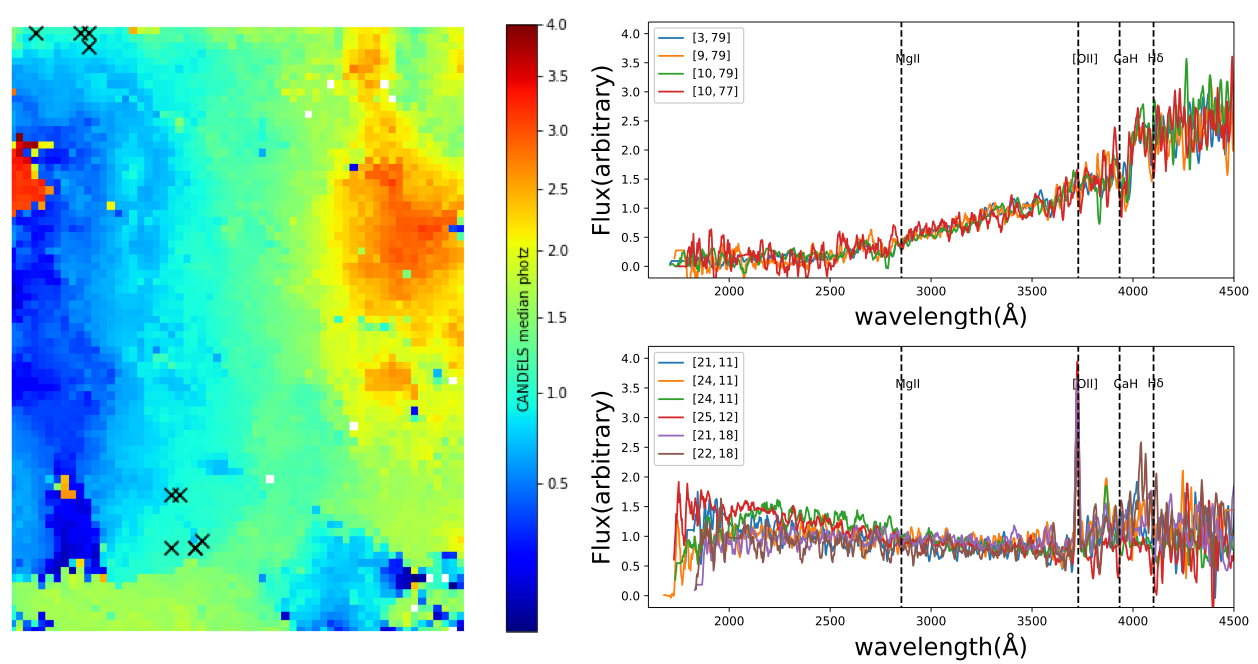
\includegraphics[width=\textwidth]{Hemmati18_Fig8_VVDS_spec.png}
%
\caption{\small \emph{Left:} A Self-Organizing Map (SOM) from
\citet{hemmati18} visualizing the relationship between galaxy
brightness in different broadband filters (projected into a two-dimensional space) and observed spectroscopic redshift (indicated by the color map).
SOMs guide the optimal construction of training samples by highlighting
which galaxy classes require targeting.  \emph{Right:} The
spectra associated with localized SOM regions have similar spectra, as well as similar redshifts. \textcolor{red}{JAN: Contra the previous text, I would say that the similarity of the spectra is neither remarkable nor surprising, since to be assigned to the same cell the galaxies have to have extremely similar SEDs, and hence spectra.  A bigger open question is can you get similar apparent SEDs from multiple redshifts (e.g., are there degeneracies with other parameters); the SOM is not necessarily one-to-one with redshift, but should be deterministic of spectral shape in any event.} }
%
\label{fig:SOM}
%
\end{figure}

The 2011 Nobel Prize in Physics was awarded for the discovery that the expansion of the universe has been accelerating instead of slowing down due to gravity as previously expected, starting when it was roughly half its current age.  This accelerated expansion is often attributed to a mysterious ``Dark Energy,'' the origin of which remains unknown.

Dark Energy is perhaps the single most important unsolved problem in both
cosmology and particle physics.  As such, it has inspired enormous
world-wide effort and the construction of dedicated ground and
space-based facilities.  These include LSST, Euclid, and WFIRST.  The
goal of these experiments is the precision mapping of cosmic structure.
Because this structure grows as the universe does, these measurements allow us to reconstruct the cosmic expansion history and distinguish amongst 
Dark Energy models.

Most cosmological probes require measurements of galaxy
``redshifts,'' the Doppler-like shift in the observed wavelengths of
emitted light; like structure on the largest scales, the wavelengths of light also grow with the cosmic expansion as it travels to us.  By comparing the relationship between redshifts and other observable quantities (such as angles or brightnesses) to expectations from cosmological models (including dark energy parameters), we can constrain the nature of our Universe.   Accurate redshifts are conventionally derived via spectroscopy by comparing the observed wavelengths of
spectral features to the characteristic wavelengths of those features where light was emitted.  Less precise redshifts, called ``photometric redshifts'' (or photo-$z$s), can be obtained from imaging (a.k.a. ``photometric'') data
alone, a compelling option for large and faint data sets where
spectroscopic redshifts are infeasible.  However, ``to infer cosmological
parameters not limited by systematic errors, accurate redshift
measurements are needed'' \citep {hemmati18}.  

Spectroscopic redshifts are critical for both the training of
photometric redshift algorithms and for calibrating results in order to
correct for biases.  Complete photo-$z$ training samples can
\emph{increase the Dark Energy Figure of Merit in LSST by 40\%}
\citep{newman15} and Keck-FOBOS is particularly powerful in this respect
because it has no redshift desert.  Keck-FOBOS can measure spec-$z$s
above $z > 1.5$ via rest-frame UV features, eliminating the need for
expensive, space-based near-IR spectroscopy.

\medskip
%
\chal{photozs}
%
\noindent {\bf Data-Science Challenge \ref{photozs}: Enable High-precision LSST
Photometric Redshifts ($\sigma_z/(1+z) \lesssim 0.02$ at i(AB) $<$
25.3) with Targeted Training Spectroscopy}.  Delivering optimal photometric redshifts with minimal errors per object will require sets of $>10,000$ spectra for training purely machine learning-based algorithms or optimizing our knowledge of galaxy spectra and calibration errors for template-based and hybrid algorithms.  Our proposed FOBOS instrument is ideally suited to providing this training set, considering  the requirements in \citet{newman15}.  Our goal is to design and deliver an optimized set of spectroscopic redshifts which will enable photometric redshifts to be accurately 'painted on' to LSST imaging-only objects, and thereby improve both dark energy and galaxy evolution science from LSST.


%, but a complete program would
%require a 400-night investment in 10 m telescope time.  This challenge
%demands a reduction in the required FOBOS training sample by a factor of
%$\sim$4 via clever application of state-of-the-art machine learning
%techniques.
% JAN: I don't agree with that text, but also think it's way down in the weeds for a pre-proposal.  
%Neural network trained photo-$z$s have long been recognized for
%providing the best precision when sufficient training sets are available
%\citep[e.g.][]{bundy06}, and significant effort is underway in
%optimizing their application to future cosmological imaging surveys.
% JAN:  NNs are not necessarily leading the field right now, but they also don't solve this issue.  The requirement is set based on being able to obtain a <0.002(1+z) calibration from the training set if redshift success is high.  
%\citet{hemmati18} for example have exploited Self-Organizing Maps (SOMs,
%Fig \ref {fig:SOM}) to sort multiband photometric data by observed
%redshift in order to select optimized training samples for spectroscopic
%followup.
% JAN: That does not change the math for direct calibration, which the SOM fundamentally is doing..



\subsubsection{A Comprehensive Picture of the Proto-galaxy Ecosystem}
\label{sec:galaxies}
\noindent \comment{1 page}

Roughly 4 billion years after the Big Bang ($z \sim 2$), the universe
entered a key epoch in which proto-galaxies transitioned from
interacting, gas-rich systems into the more ordered, star-dominated
structures that populate the universe today.  This period marks the peak
of global star formation rate and galaxy assembly history.   To
understand it, we must not only study the galaxy population at this
epoch but the entire galaxy ``ecosystem'' which includes their
gas-filled environments.  The goal is to build a comprehensive picture
of the physical processes that fuel proto-galaxy growth, shape their
internal structure, and influence their environment.

LSST's panoramic imaging will detect huge numbers of galaxies at this
epoch.  Targeted followup with Keck-FOBOS will allow us to ascribe
detailed galaxy and environmental information from deep spectroscopic
training samples to the much larger cosmic volumes surveyed with
broad-band imaging.

\begin{figure}[h!]
%
\vskip -0.1in
%
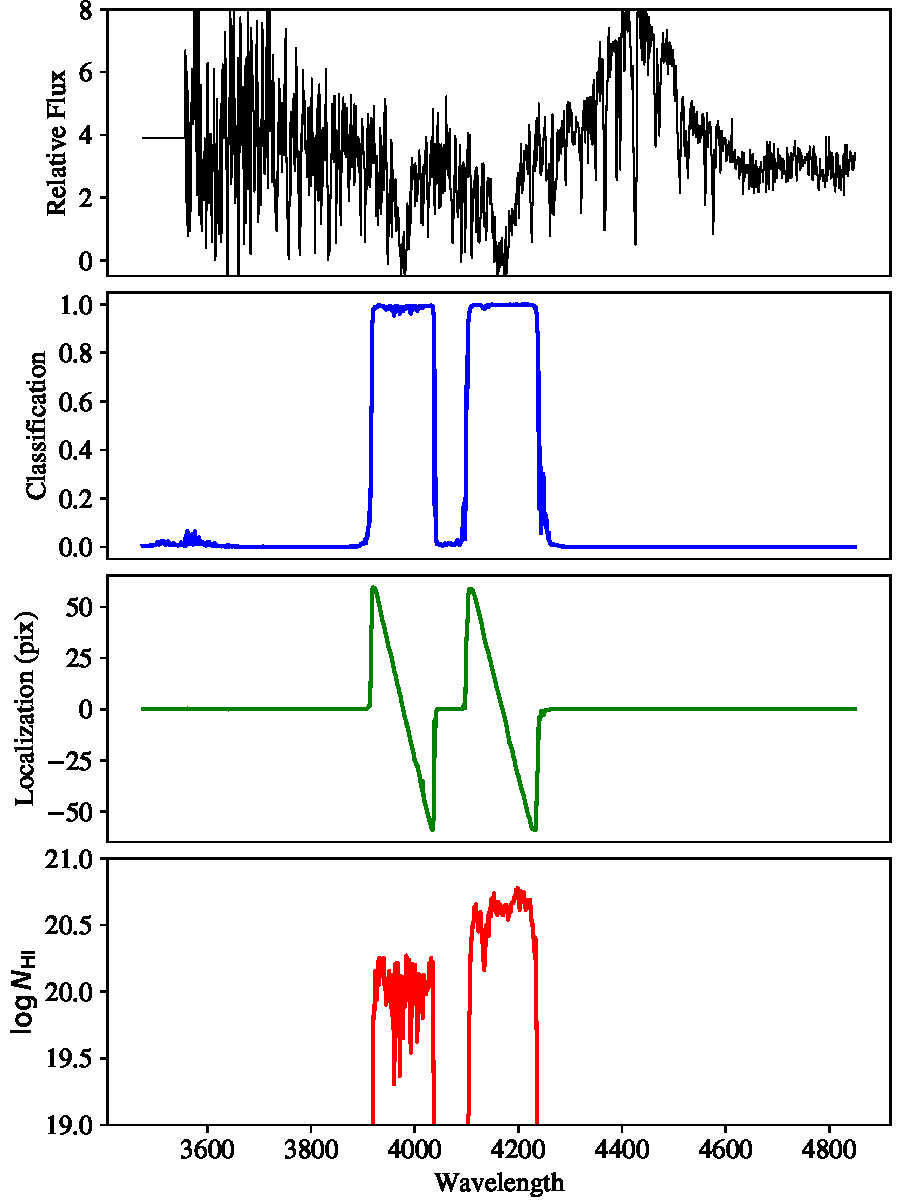
\includegraphics[width=0.5\textwidth]{Parks18_Fig7_fig_labels.pdf}
%
\caption{\small Example of machine learning applied to absorption
features in rest-frame UV spectroscopy to detect two intervening gas
clouds along the line-of-sight \citep[from][]{parks18}.  A spectrum is
shown at top with lower panels indicating associated labels conveying
physical information.  Keck-FOBOS will provide a rich set of similar
features and the opportunity to transfer labels to imaging and higher
redshift data sets.}
%
\label{fig:absorber}
%
\end{figure}

\medskip
%
\chal{phot}
%
\noindent {\bf Data-Science Challenge \ref{phot}: Apply Deep Learning to
infer star formation rates and formation histories, dust content, wind
properties, and stellar masses from $z \sim 2$ photometry}.  The range
of observed spectral types is remarkably constrained by broad-band
imaging (Figure \ref{fig:SOM}, right panel), suggesting a far greater
potential for imaging data to reveal physical properties with sufficient
training than conventional modeling of spectral energy distributions
(SEDs) would suggest.  Applying machine learning, our challenge is to
deliver SDSS-like information for millions of imaged galaxies at $z \sim
2$.  With simulated data sets, we will investigate derived uncertainties
and biases and explore benefits from incorporating additional imaging
information like morphology, structure, and size from a wide range of
wave-bands (e.g., LSST plus Euclid plus WFIRST).  The exercise will
define requirements for Keck-FOBOS instrument performance and the FOBOS
Public Survey design.

\medskip
%
\chal{uv}
%
\noindent {\bf Data-Science Challenge \ref{uv}: Enable label transfer
from rest-frame optical to UV stellar and ISM indicators}.  There are
many powerful gas and stellar spectral features just redward of the
Lyman-$\alpha$ line at 1216 \AA.  By combining Keck-FOBOS UV and near-IR
spectroscopy (e.g., from PFS) at $z \sim 2$, we can transfer ``labels''
best modeled in the rest-frame optical to spectra at UV wavelengths, at
least for certain types of galaxies.  This ``label transfer'' will
dramatically enhance interpretation of JWST discoveries of the first
galaxies ($z \sim 10$) for which rest-frame UV imaging and spectroscopy
will be most accessible.  A similar application can ascribe the escape
fraction of Lyman continuum radiation observed in the Keck-FOBOS Public
Survey to constrain the sources responsible for ``reionization'' at $z
\sim 6$.  With simulated spectral observations, we will determine the
extent of label transfer that is possible and set requirements on
training samples.


\medskip
%
\chal{lowsnr}
%
\noindent {\bf Data-Science Challenge \ref{lowsnr}: Train short
spectroscopic exposures in combination with LSST photometry to provide
environmental diagnostics for 1M galaxies at $z=1$--$2$}.  Photometric
redshifts, while acceptable in large cosmological analyses, wash out
information about the local position of galaxies with respect to one
another.  To characterize a galaxy's local environment and identify its
neighbors requires (observationally expensive) spectroscopic redshifts
(spec-$z$s).  However, with improved photometric redshifts available
from Challenge \ref{photozs} and strong priors on spectral types
(Challenge \ref{phot}), machine learning techniques can yield
\emph{spectroscpic} redshifts at much lower signal-to-noise than
conventional redshift measurements. Specifically, our challenge is to
develop a methodology that can measure 300 km s$^{-1}$ accuracy
spec-$z$s on spectra obtained in just 10 minutes with Keck-FOBOS.  This
would enable an SDSS-like environmental study of 1M galaxies at
$z=1$--$2$ in just 20 nights of 10 m telescope time, making it a
compelling sub-component of the Keck-FOBOS Public Survey.






%\begin{wrapfigure}{r}{0.6\textwidth}\small
%%
%\includegraphics[width=0.6\textwidth]{TestBench.jpg}
%%
%\caption{\label{fig:testbench} A schematic of the current UCO fiber test
%bench.  The components to the right of the first fiber positioner will
%be repackaged and delivered to Keck for our on-sky experiment; the
%fibers themselves will be fed light from Keck after being plugged into a
%DEIMOS mask.  Image Credit: Jaren Ashcroft.}
%%
%\end{wrapfigure}


% \begin{wrapfigure}{r}{0.5\textwidth}
%  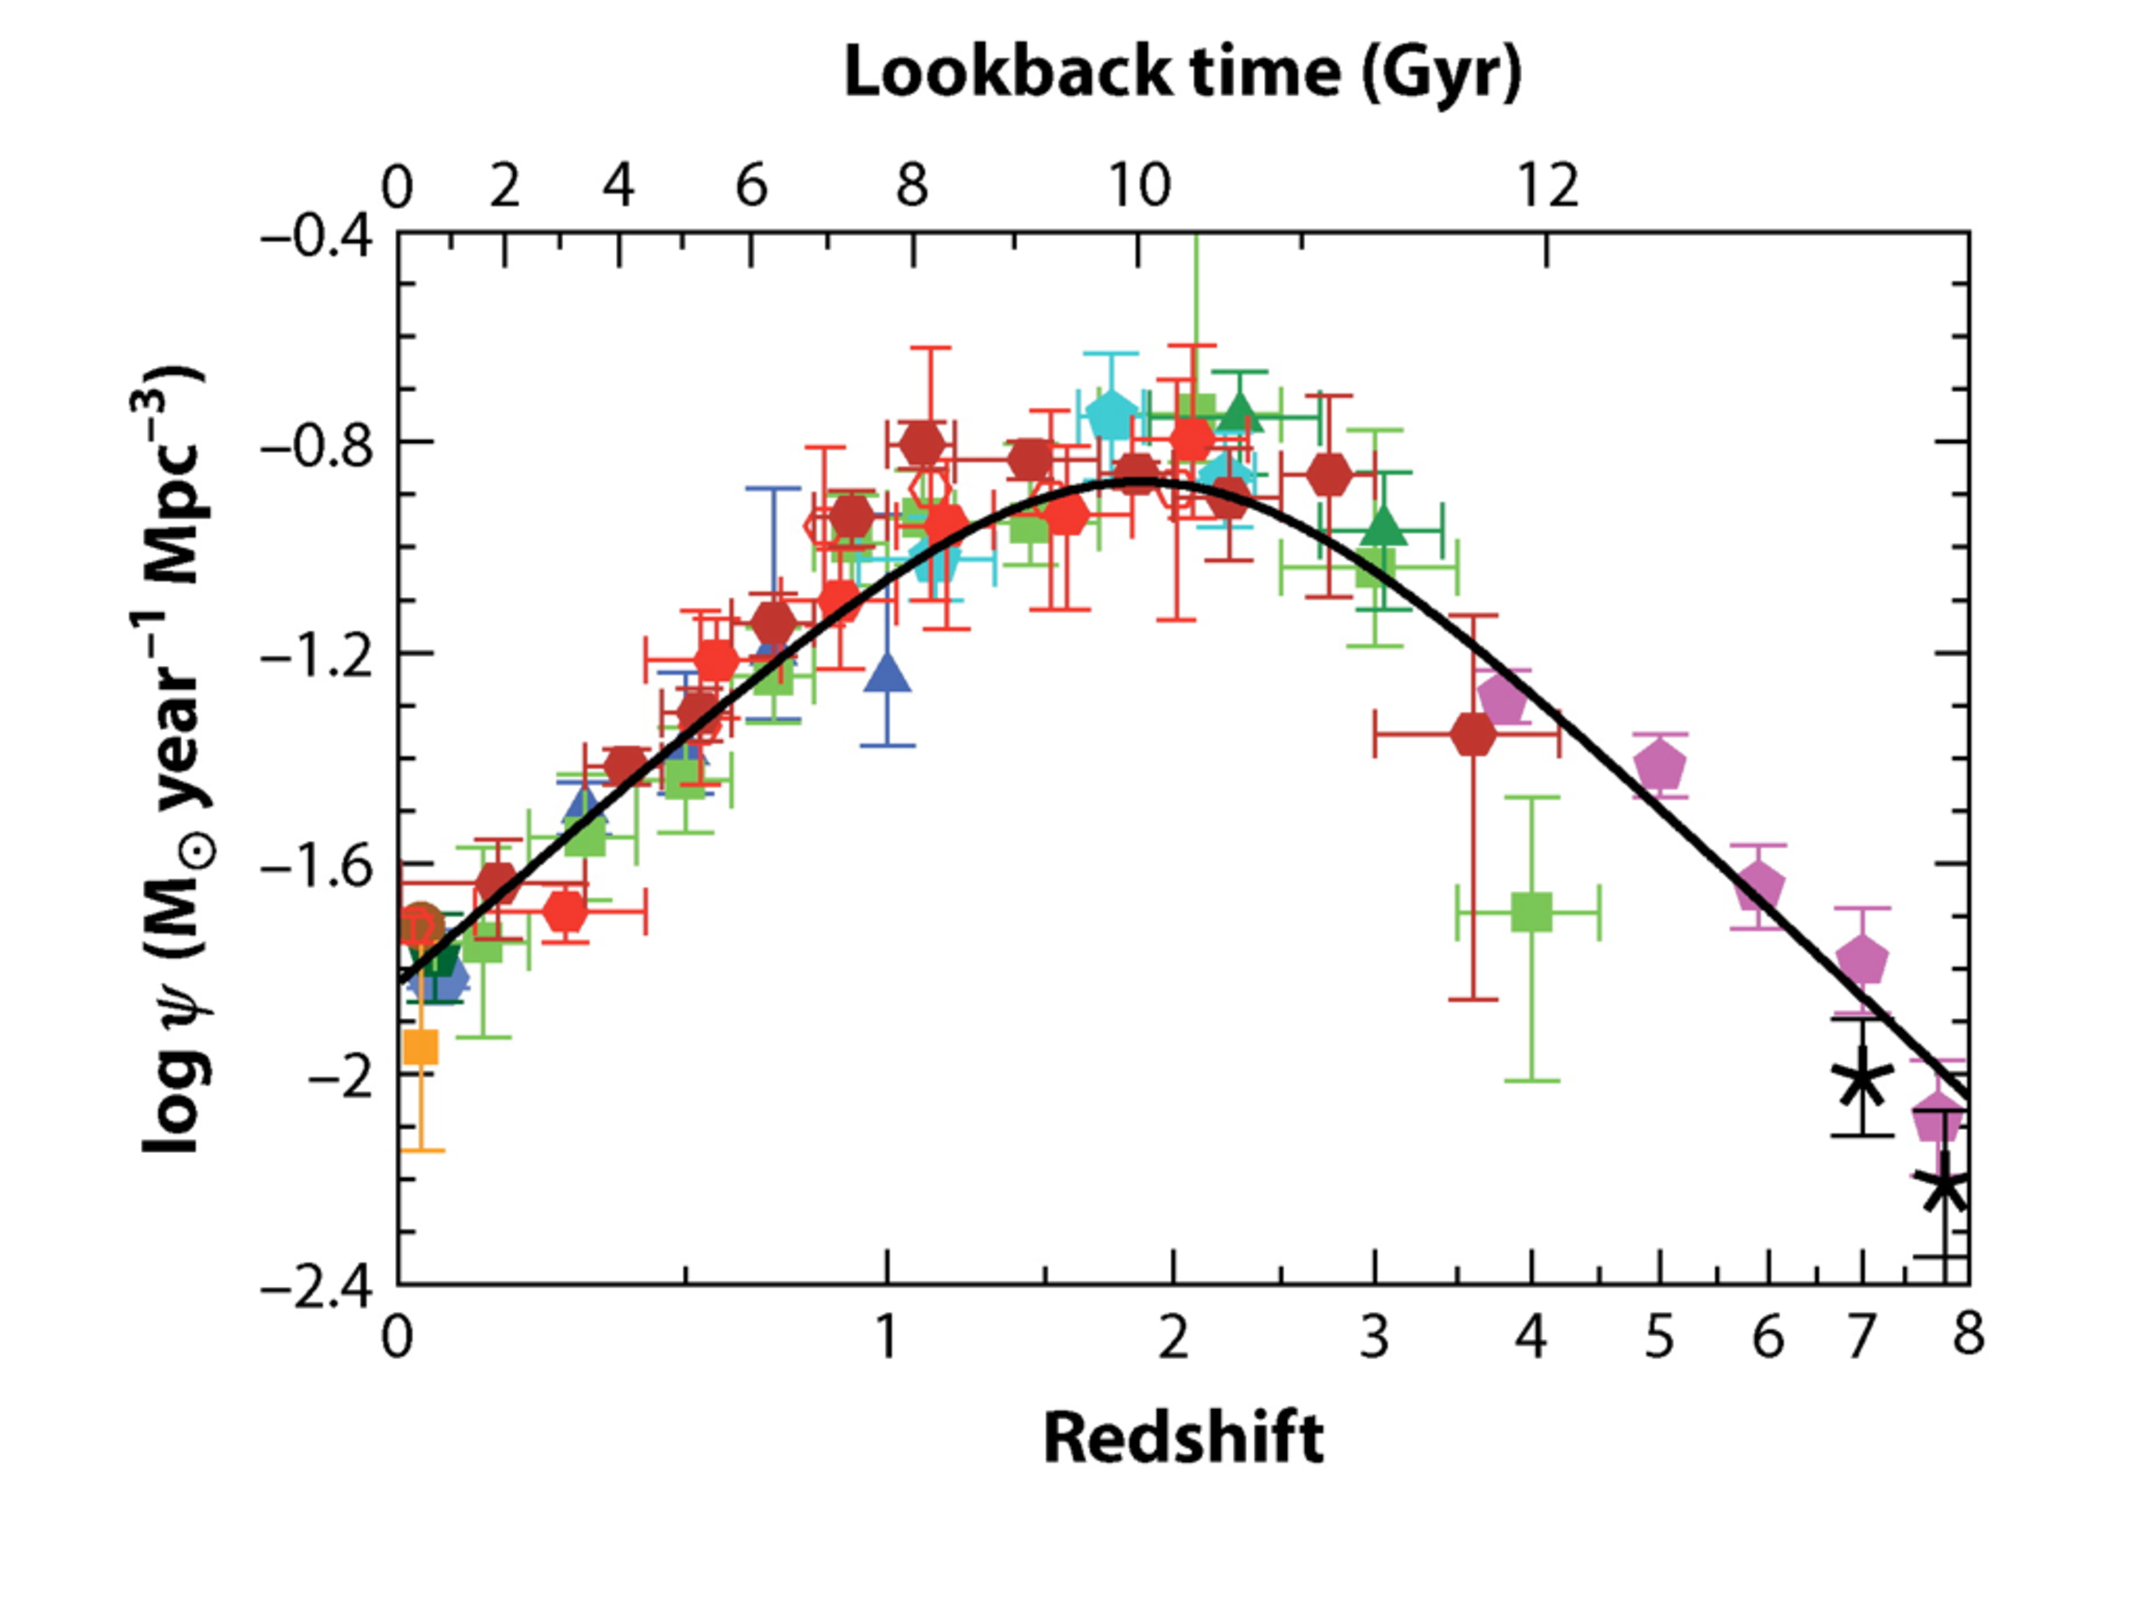
\includegraphics[width=0.5\textwidth]{madau_plot.pdf}
%  \caption{\small From Madau \& Dickinson (2014) }\label{fig:Madau_plot}
% \end{wrapfigure}

%A critical transition in evolution of galaxies in our Universe emerges
%when one considers the volumetric star-formation rate as a function of
%cosmic time 
%
% - cosmic star-formation rate shows the unique phases of the growth of
% galaxies in the Universe
%
% - the detailed cause for the decline in the CSFR since z~2 remains
% unclear, but it could be thought of as the starvation of galaxies from
% the rapid gas accretion they enjoyed in the early universe.
%
% - the outbreak of star-formation sparked by free-falling accretion of
% gas is now stymied by the size of the galaxies themselves.
%
% - a number of fundamental properties of galaxies have emerged over the
% past ~30 years: mass, size, metallicity, star-formation rate, angular
% momentum, and gas fraction.  Environment
%
%
%The rate at which stars have been born in the Universe has varied
%dramatically over cosmic history.  At roughly half its current age, the
%Universe was on average forming 10 stars for every one star formed
%today \comment{ref}.  At these epochs, galaxies looked rather different
%then they do now, dominated by all-consuming star-formation regions
%\comment{ref}.  These morphologies are only seen in rare star-burst
%galaxies in the Local Volume \comment{ref}.  The 

\begin{figure}[h!]
%
\vskip -0.1in
%
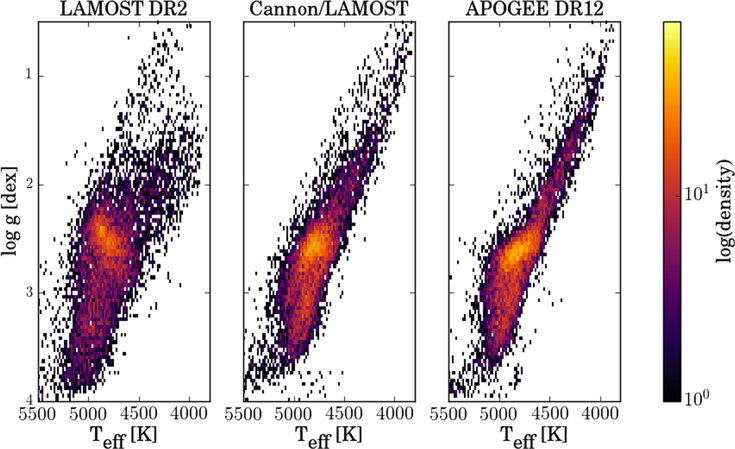
\includegraphics[width=\textwidth]{CannonLAMOST.jpg}
%
\caption{\small Verification of application of {\it The Cannon} to
LAMOST spectra based on stellar paremters determined by the
high-resolution APOGEE data from Ho et al.\ (2017).  Each panel shows
the derived effective temperature, $T_{\rm eff}$, and surface gravity,
$\log g$, for each star, with the color representing the density of
stars at each position.  The left panel shows the results for the LAMOST
spectra using a direct fitting approach, the right panel shows the
results derived from the high-resolution APOGEE data, and the middle
panel shows the results of using {\it The Cannon} to determine the
stellar parameters using the low-resolution LAMOST spectra trained by
the APOGEE-derived parameters.  Results from {\it The Cannon} are more
accurate and astrophysically plausible.}
%
\label{fig:Cannon}
%
\end{figure}

\subsubsection{Unraveling the Formation History of our Local Group of Galaxies}
\label{sec:localgroup}
\noindent \comment{1 page}

While only a single realization of the galaxy-formation process, our
Local Group provide unparalleled opportunities to study galaxies in
exquisite detail, by virtue of being able to spatially resolve their
constituent parts.  In fact, the Gaia satellite (ref) is currently
revolutionizing our understanding of our Milky Way Galaxy, providing
distances and on-sky motions for more than a billion stars spanning the
full extent of its disk.  These data represent a gigantic leap forward
in our ability to construct a history of the Milky Way by effectively
tracing its stellar populations and dynamical structures back in time.
However, the Gaia data are still limited: Fewer than 10\% of stars will
have a full complement of three-dimensional space motions, fewer than
0.3\% will have the basic stellar parameter measurements needed to
classify the stellar type, and only 0.1\% will have measured chemical
abundances.  Existing and ongoing surveys, like SEGUE, RAVE, and APOGEE,
and planned surveys, like WEAVE and 4MOST (refs), provide critical
supplementary observations, but these efforts only just begin to fulfill
the potential of the Gaia astrometric data.  Directly observing the all
1.7 billion stars is simply untenable for the foreseeable future.

Instead, a growing number of studies aim to infer the necessary
measurements using novel applications of machine-learning.  For example,
Ness et al.\ have developed {\it The Cannon}, a supervised learning
algorithm that uses spectra with known stellar parameters to label
spectra where those parameters are unknown.  In one application, they
determined three fundamental parameters for 55000 APOGEE spectra using a
1\% training sample.  Additionally, Ting et al.\ have developed {\it The
Payne}, which uses a neural network and theoretical stellar spectra to
determine 25 stellar labels.  In both of these applications, careful
attention has to be given to the limitations of the training sample,
similar to the SOM example provided in Figure 1.  At their core,
machine-learning algorithms, particularly supervised learning, are only
as good as the parameter space spanned by their training sets.

\medskip \chal{gaia} \noindent {\bf Data-Science Challenge \ref{gaia}:
Stellar parameter determinations for a billion stellar spectra.}  To
realize the full potential of the Gaia astrometric catalog, one needs
the full 6D phase space for each star and its chemical abundance
pattern.  Although anything more than simple total metallicity
measurements are out of reach for FOBOS, a strategically developed
training set observed at high S/N can be used for kinematics and simple
stellar parameter determination.

% Beyond its internal chemodynamical history, LSST will also reveal
% hundreds of faint Milky Way satellites, as well as discover new
% satellites of the Andromeda and Triangulum galaxies, extending the
% census of these galaxies.  These faint galaxies provide critical tests
% of the hierarchical formation of the Local Group.

% \medskip \noindent {\bf Data-Science Challenge 7: Dynamics of newly
% discovered Ultra-Faint dwarfs.}

\subsubsection{Time Domain}
\label{sec:timedomain}
\noindent \comment{1/2 page}



\section{Project Implementation}
\label{sec:project}

This proposal involves three coordinated activities: 1) Organizing and evaluating the results of a community-wide
effort to address simulated Data Science Challenges; 2) Completing Preliminary Design for the Keck-FOBOS
instrumentation, informed in part by refining requirements as a result of (1); 3) Designing the operational modes,
planning tools, data analysis software, and serving platforms necessary for delivery of public training sets.
Anticipating significant progress in all three activities, we will request NSF MSRI-2 funding in 2021 to build and
deploy Keck-FOBOS at the telescope, carry out required observations, and publicly serve the data products.  FOBOS would
see first light in 2027 and carry a total cost of \$32M (without contingency in 2019 dollars).  While we focus the
current request on work required for the Preliminary Design Phase, we outline the overall project plan and final
deliverables in order to motivate this work.

\subsection{Keck-FOBOS Instrument Concept}
\label{sec:concept}
% \noindent \comment{1 page}

% Here's an alternative way to put in figures if we want captions on the side (to save space)
% Could introduce a new ``counter'' to count and label figures appropriately
\centerline{\hbox{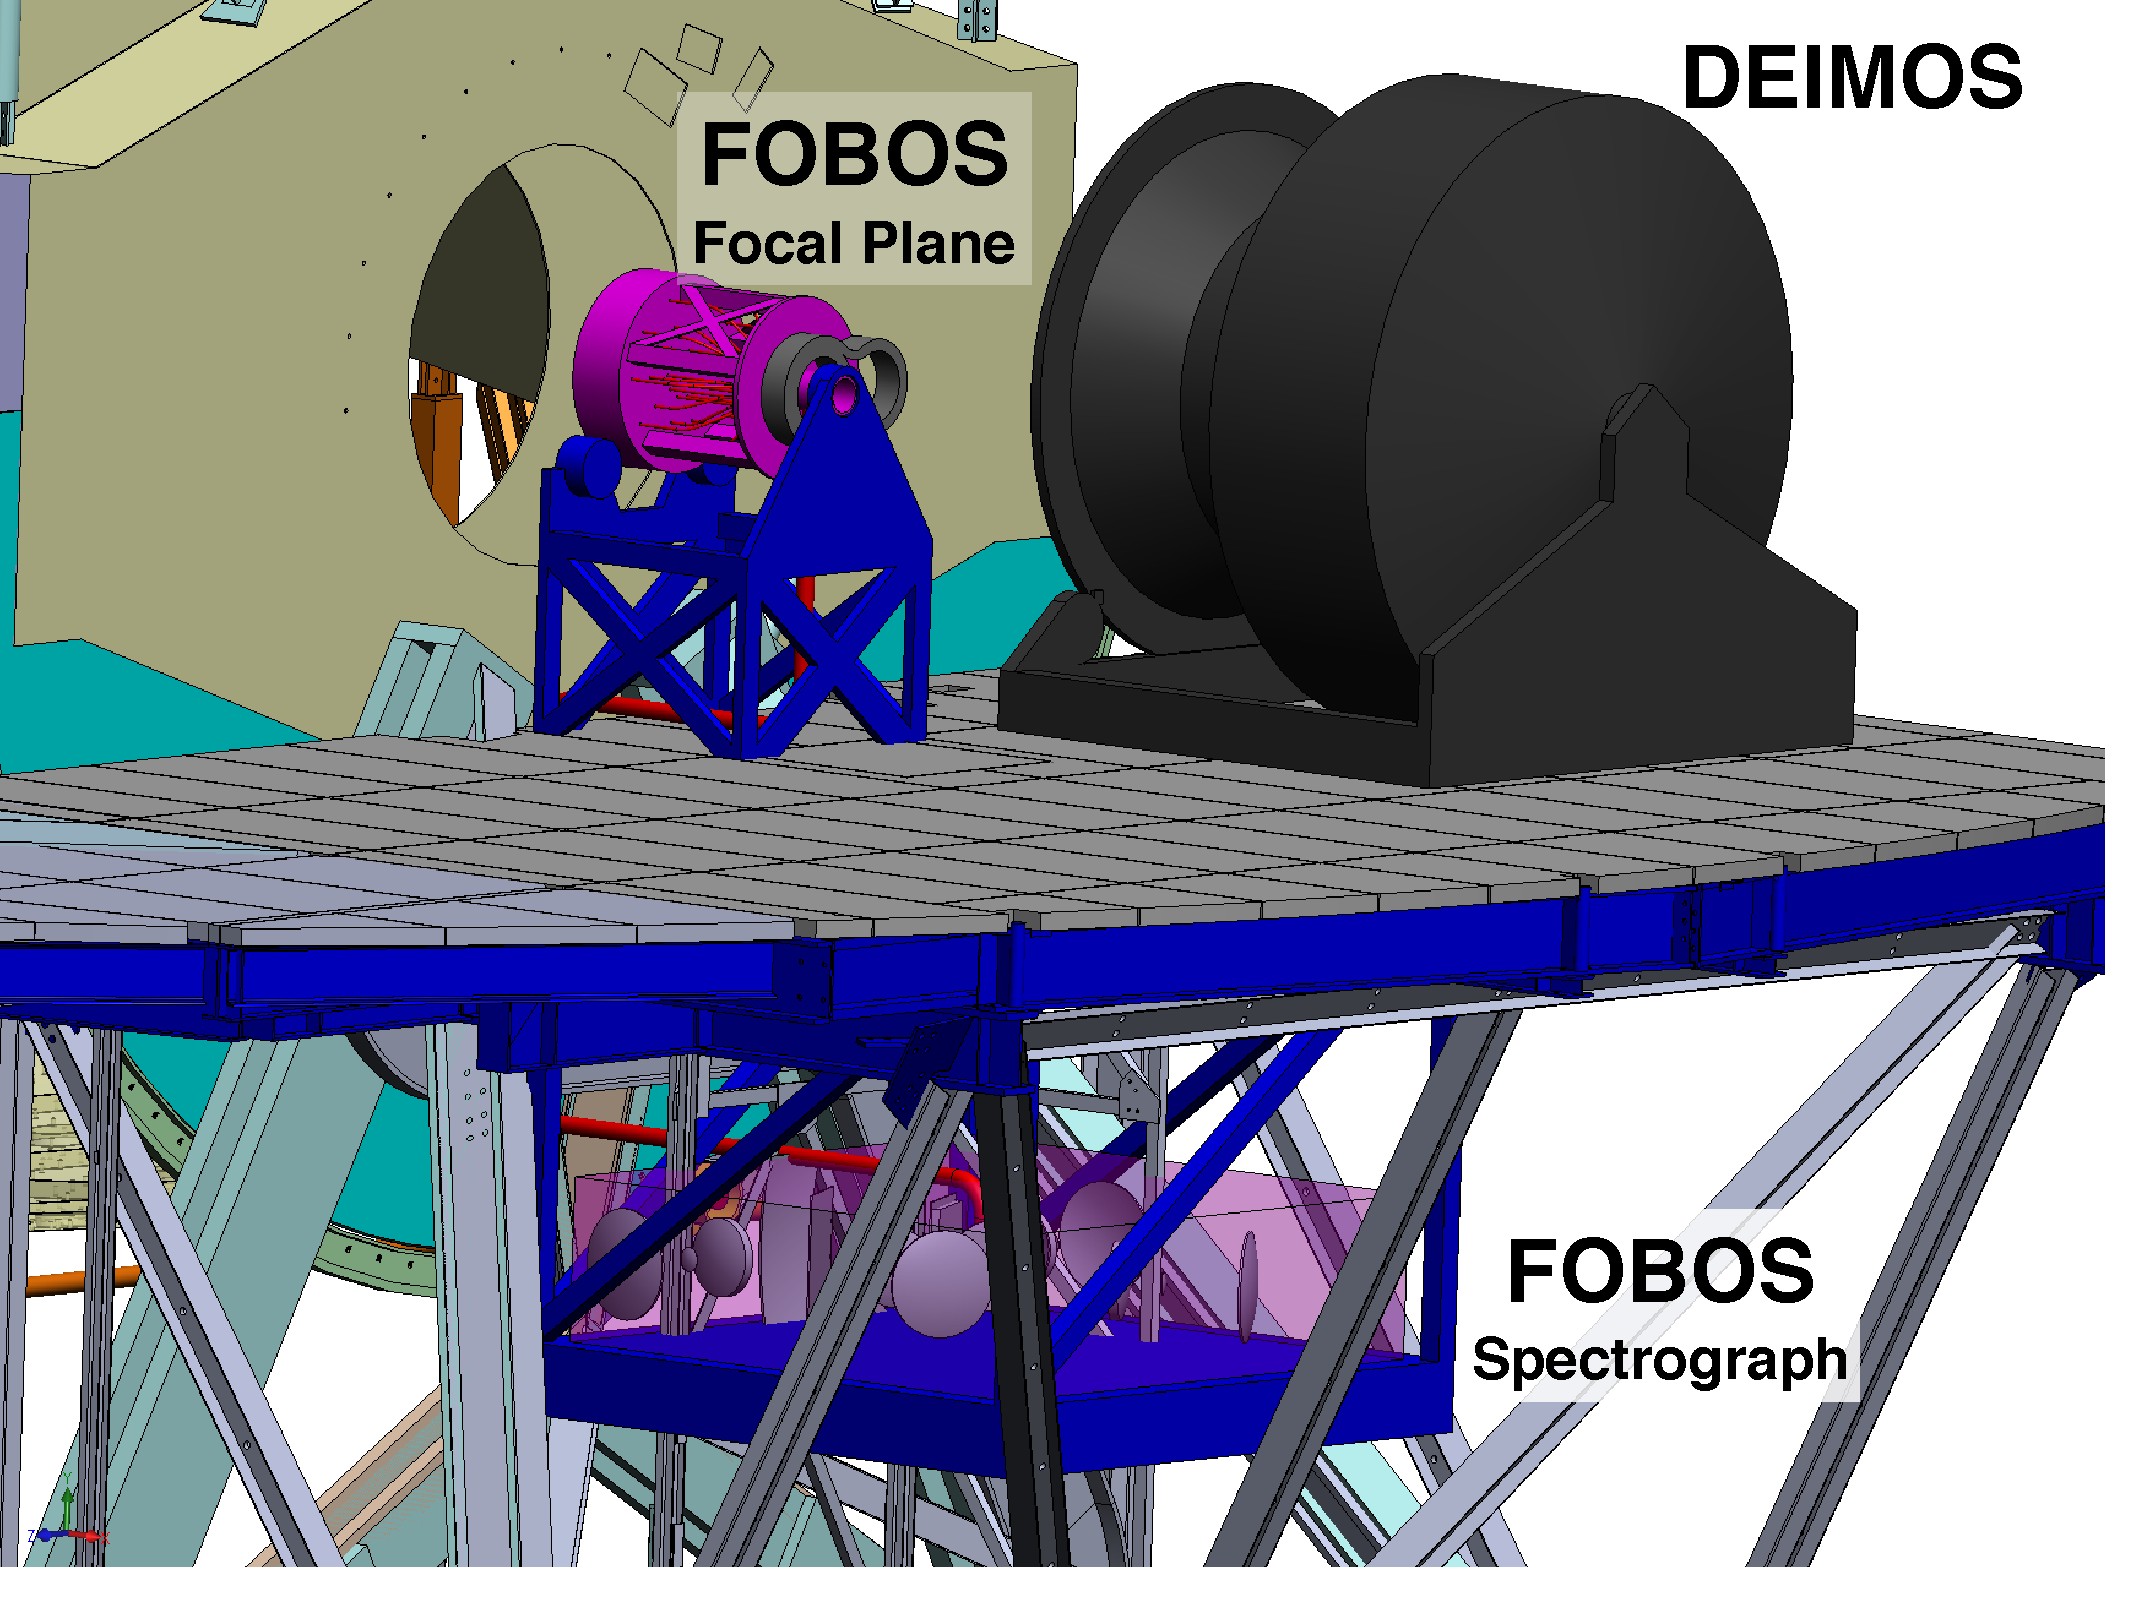
\includegraphics[width=0.6\textwidth, angle=0]{FOBOSatKeck_v1.pdf}
    \hspace{0.1cm} \vspace{2in}
    \parbox[b]{0.3\textwidth}{\small {\bf Figure ??:} Rendering of FOBOS instrument systems deployed at the Keck II Nasmyth port.  By mounting the FOBOS spectrographs under the Nasmyth platform, other instruments like DEIMOS can maintain access to the telescope. \vspace{2cm}}}}



% \begin{figure}[h!]
%  \vskip -0.1in
%  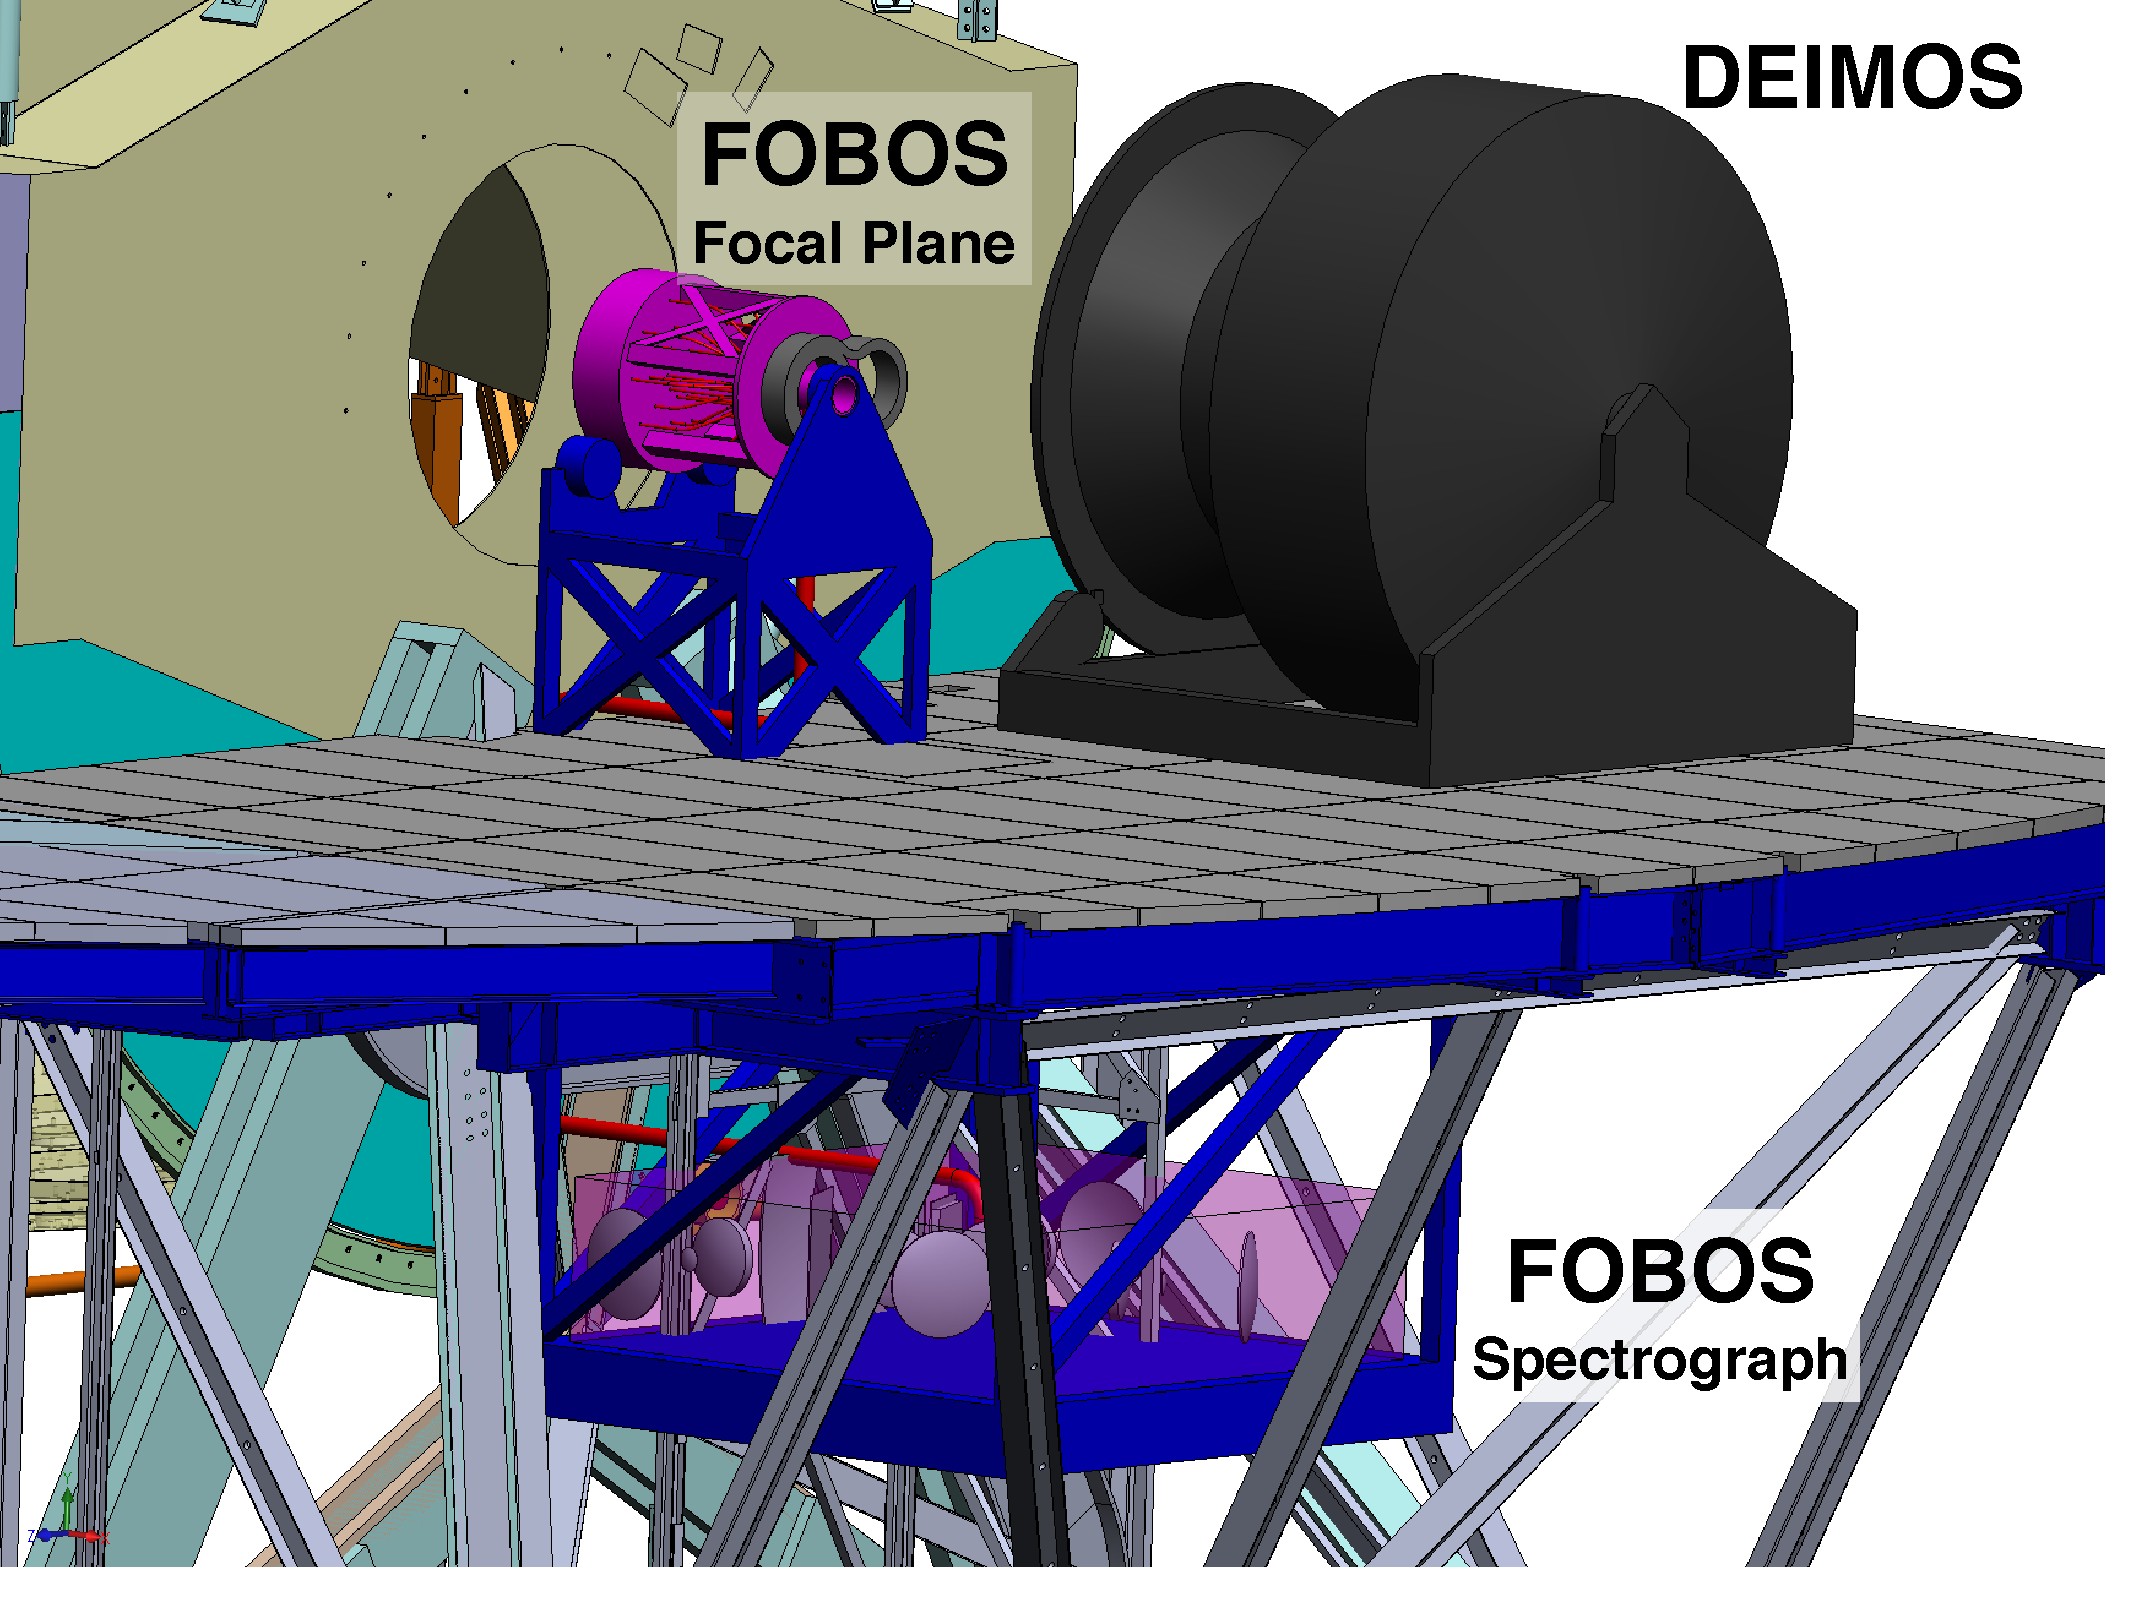
\includegraphics[width=\textwidth]{FOBOSatKeck_v1.pdf}
%  \caption{\small Rendering of FOBOS instrument systems deployed at the Keck II Nasmyth port.  By mounting the FOBOS spectrographs under the Nasmyth platform, other instruments like DEIMOS can maintain access to the telescope.}\label{fig:layout}
% \end{figure}

Mounted at the Keck II Telescope's Nasmyth focus, the Fiber Optic Broadband Optical Spectrograph (FOBOS) will be one of
the most powerful spectroscopic facilities in the next decade.  FOBOS consists of several key components (Fig
\ref{fig:layout}).  A compensating lateral atmospheric dispersion corrector (CLADC) ensures that target light from all
wavelengths falls on allocated fibers while also correcting image aberrations at the edges of the 20 arcmin diameter
Keck field that result from the telescope design.  The final lens surface in the 3-lens CLADC also serves as the
mounting plate for roaming Starbugs fiber positioners.  Starbugs patrol a large on-sky area, enabling flexible
targeting configurations that can be dynamically adjusted during observations.

A total of 1800 150 $\mu$m core diameter fibers are deployed at the curved focal plane, which rotates and translates to
maintain image positions as the telescope tracks across the sky.  The fiber run is kept at less than $\sim$10 m to
maintain high throughput at UV wavelengths, and special care is given to stress-relief cabling to minimize variable
focal ratio degradation over the fiber run.

Sets of 600 fibers feed each of three identical spectrographs.  Each spectrograph uses a series of dichroics to divide
the fiber output into four wavelength channels with combined coverage from 310 to 1000 nm and mid-channel spectral
resolutions of $R \sim 3500$.  The dispersed light in each channel is focused by an f/1.1 catadioptric camera and
recorded by an on-axis CCD mounted at the center of the first camera lens element.  Spectrographs are mounted in a
temperature controlled housing installed under the Nasmyth Deck to allow space for other Keck instruments to access the
Nasmyth port.  The end-to-end instrument throughput is greater than 30\% at all wavelengths.

FOBOS includes observatory level systems for precise instrument calibration using dome-interior screen illumination, a
metrology system for accurate fiber positioning, and guide cameras for field acquisition and guiding.  The instrument
design envisions future upgrades including alternate collecting modes that deploy multiple fiber bundles, feeds to
other fiber-based spectrographs at different wavelengths or spectral resolutions, and the ability to support and
benefit from image corrections with Ground-Layer Adaptive Optics.



\subsection{Keck-FOBOS Instrument Design Effort}
\label{sec:design}
% \noindent \comment{1 page}

Keck-FOBOS will complete its current conceptual design phase in October 2019.  Funding from this proposal will support preliminary design beginning in November 2019.  A detailed schedule of activities is attached.  Major components of the preliminary design effort are described below.

\noindent \textbf{Atmospheric Dispersion Compensator (ADC).} The opto-mechanical design, tolerancing, lens cell design, motion systems, and software controls design of the ADC will be completed.  We will complete a competitive bid selection of optics vendors so that upon passing the the FOBOS Preliminary Design Review (PDR), large lens procurement can begin immediately.  This procurement is a long-lead item in the overall schedule.

\noindent \textbf{Focal Plane System.} The final ADC lens element serves as the focal plane mounting plate for the fiber positioners.  This focal plane system must rotate and translate to track the field and refraction angles from the ADC.  Mechanical design, including flexure analysis and the selection of drive mechanisms and vendors will be completed.  This system also defines one of the interfaces to the Keck Telescope and must comply with Keck Observatory space envelopes, servicing needs, and other requirements.  The focal plane system also interfaces with guide cameras for field acquisition and guiding.

\noindent \textbf{Starbugs fiber positionsers.} Starbugs are a positioning technology developed and deployed by the
Australian Astronomical Observatory (AAO) which has partnered with our team to generate a conceptual design for
Starbugs in the context of FOBOS.  Design requirements for Starbugs in FOBOS are more relaxed than the currently on-sky
TAIPAN instrument thanks to the larger physical plate scale at Keck.  AAO will serve as a vendor during preliminary
design but is interested in exploring a partnership and in-kind contribution model in the construction phase.  In addition to the Starbugs themselves, a fiber metrology system (for accurate closed-loop positioning) will also be developed.

\noindent \textbf{Fiber System.} We will complete the optical design and processing plan for affixing forward optics
lenses to each fiber's head (these demagnify and speed up the beam for proper fiber coupling).  A micro-lens array
solution will be developed for a central, fixed-position 4.5-arcsec diameter IFU for fast source acquisition.  With vendors selected, we will be ready to begin prototyping.  We will
research anti-reflective coating vendors and options and detail throughput and stress performance specifications.  This
workpackage also includes the stress-relief cable system and fiber termination hardware and processing.

\noindent \textbf{Spectrographs.} The optical systems and components (slit, collimator, dichroics, gratings, and camera), an analysis of acceptable tolerances and performance, their mechanical supports, software controls, and the overall enclosure will all be advanced through preliminary design.  Vendors for major components will complete competitive bids.  Detectors, cryostats, read-out electronics and systems for thermal management will be designed and associated vendor relationships secured. We will complete a preliminary assembly and integration plan.

\noindent \textbf{Calibration System.} This package includes design of an interior dome screen and projection system for injecting calibration sources with sufficient spatial uniformity and stability into the instrument.  We will work with the Observatory to develop an integration and controls plan.  No such calibration system currently exists at Keck.

\noindent \textbf{Auxiliary Systems.} Design of auxiliary systems includes Nasmyth platform interfaces, utilities access, fiber routing and support, thermal control and vibration control systems.


\subsection{Addressing Data Science Challenges and Designing FOBOS Training Sets}
\label{sec:survey}
% \noindent \comment{1 page}

Our team includes leading experts on data science applications to astronomy and LSST specifically.  We will also use
our established connections to LSST's Informatics and Statistics Science Collaboration (ISSC) to advertise, recruit,
and coordinate efforts to tackle the Data Science Challenges described in Section \ref{sec:goals}.  Our proposal
request includes two open workshops to motivate progress and discuss results. At the end of the proposal period, we
will publish the results and developed software packages.

The Data Science Challenges require work on simulated imaging$+$spectroscopic data sets where input physical properties
(e.g., redshift) can be imposed and the output, recovered values compared against the input.  Simulated imaging data
(e.g., from LSST and WFIRST) are in-hand, while mock spectroscopy will be provided by a Keck-FOBOS instrument simulator,
an initial version of which has already been developed.  Further advances to be supported by this proposal include
improved error modeling and simulating systematic effects from detector artifacts, image quality aberrations informed
by the emerging detailed optical design, and variable observing conditions.

The resulting success in addressing each Data Science Challenge will define a level of readiness and set requirements
on the associated Keck-FOBOS training sets required, including number of sources, pointings, magnitude limits,
signal-to-noise thresholds, and observing conditions.  Preliminary observing design and a description of required
operational modes to efficiently observe these training sets will begin with this proposal.  Operational modes will set
requirements on target aggregation and prioritization systems, field acquisition speed, field rotation range, zenith
avoidance zone, reconfiguration time, calibrations, read-out time, quicklook reduction software and processing rates.
We will develop integrated program concepts that efficiently combine required observations.  Detailed survey and
execution plans will be completed in the next phase of this project (MSRI-2).  As in previous federally-funded
projects, we fully expect that Senior Personnel at Keck institutions will be successful in collaborative efforts to
secure significant amounts of telescope observing time to enable rapid, publicly release of training data with any
proprietary period waived \citep[e.g.,][]{newman13}.  

% The complete photo-$z$ training survey described in \citet{newman15} would
% require 15 independent pointings, each spanning 0.1 deg$^2$ with a target density of 6 arcmin$^{-2}$ (8 arcmin$^{-2}$
% when including $z > 1.5$ galaxies accessible in the UV with Keck-FOBOS), perfectly matched to the Keck-FOBOS
% field-of-view and target density.  With a conservative exposure time of 100 hours to reach 75\% redshift completeness
% for 40,000 galaxies with $i_{\rm AB} < 25.3$, the Neman survey would require 400 nights.  Challenge \ref{photoz} would
% reduce the required survey duration by a factor of at least four.  Meanwhile the extreme depths and flux-limited
% selection are likely also requirements for training sets associated with Challenges \ref{phot}, \ref{uv}.

% A wider and shallower survey component is envisioned for Challenges \ref{lowsnr} and \ref{gaia}.  With 10-minute
% integrations, a 52 deg$^2$ Keck-FOBOS sample of environmental diagnostics for 1 million galaxies could be carried out
% in less than 20 nights.  This program would sample at $z \sim 1.5$ the same cosmic volume as SDSS.  A program of a
% similar scale would provide training set data for inference of stellar parameters in the Milky Way.  These shallow programs would be integrated with the deeper components described above into a single survey plan.



% The components of the FPS are as follows:
%     - Photo-z training samples (Newman, Masters)
%         - z>1.5 in the blue
%         - z<1.5 in the red
%     - Ly continuum
%         - z~2 in the blue
%         - z~7 in the red
%     - Machine-learning the SDSS but at z~2


\subsection{Target Allocation with Artificial Intelligence}
\label{sec:targeting}
% \noindent \comment{1/2 page}

Traditionally, target allocation involves laborious hands-on
optimization of a set of desired targets, the allowed positions of
entrance apertures, and constraints on the pointing center for precise
target acquisition and tracking.  These activities are typically
preformed days in advance of any observations and inflexible to the
actual observing conditions or any real-time decision making on the
observing night.  This inflexibility can be hardware related, such as
the pre-drilled metal sheets used to provide fiber entrance apertures in
SDSS, or software related, such as with interfaces that are overly user
intensive.

For both our public survey and its long-term operation, FOBOS will avoid
these limitations and allow for fast, dynamic reallocation of fibers to
maximize its efficiency.  First, we use the Starbugs positioning system
to largely mitigate the hardware limitations to FOBOS's flexibility to
real-time reallocation of fibers.  Second, as another data-science
challenge, we will develop software that efficiently optimizes targets
for allocation given a database of sources to be observed, the aggregate
data quality for the spectra obtained of the target using a quick-look
reduction package, {\it and real-time assessments of the observing
conditions.}  Finally, each target will have an expected data quality
metric that will be used to decide when the observation has successfully
met the observing request allowing for reallocation of individual
fibers.

\medskip \chal{target} \noindent {\bf Data-Science Challenge
\ref{target}: Intelligent target allocation algorithms that integrate
multiple observing programs and reallocate fibers based on real-time
assessments of observing conditions and the aggregate data quality of
each target.}  FOBOS will generally be able to optimize observations for
multiple programs with vastly different target densities and
exposure-time requirements.  We will build a database with efficiency
and observing success metrics and aggregate data quality for all targets
that have been observed.  Queries to this database will allow the
software to learn which observations should be successful, among all
possible observations for any given pointing and observing night.  For
example, if conditions are slightly less than optimal, the Starbugs
would quickly be reconfigured to target brighter objects in a given
field.  During survey operations, we expect this to be the primary mode
of allocating fibers; however, we will also provide a PI override for
specific targets and allow for unallocated fibers to be assigned to
targets drawn from an observatory-level ``filler" database.

%   - maintains a database with observational progress on individual
%     targets in the survey and
%   - dynamically reallocates fibers based on real-time assessments of
%     the aggregate S/N of each target to meet the specific need of each
%     science case.

% This requires significant design and testing of a combined software
% package and hardware interface.  Specific considerations involve (1)
% fast and robust reduction procedures (cf. MaNGA DOS) that can assess
% the aggregate data and (2) a responsive database with a schema
% optimized for real-time decision making to select targets for
% (re)acquisition while accounting for collision limitations.  Provided
% enough design effort, this lends itself to a machine-learning
% application.

\subsection{Publicly Available Automated Data Products}
\label{sec:DAP}
% \noindent \comment{1/2 page}

The typical proprietary period for raw data acquired at Keck is 18
months.  However, typical of other public surveys (e.g., SDSS), this
period will be shortened to one year for the FOBOS Public Survey.

Both as part of our design effort and for long-term use, we will develop
a data-reduction pipeline, building on work already done for other
fiber-based observations, like SDSS and DESI.  This software will
provide both the quick reduction assessments needed for our dynamic
targeting system and the more detailed reduction to produce the data for
scientific analysis.  Reduced data will be delivered to the community
(e.g., via the Keck Observatory Archive) after the proprietary periods
are finished for {\it both} PI-led and public survey observations.

Finally, we will also provide a data-analysis pipeline that provides
high-level data products.  There are two aspects to analysis of the
data.  First, we will provide software to perform the traditional
measurements of properties like Doppler shift, emission-line strengths,
and internal kinematics that are measured from FOBOS-observed spectra.
This software will build on existing software we have built for the
SDSS-IV MaNGA survey (Westfall et al.), and it will be executed for {\it
any} data taken with FOBOS and released along with the reduced spectra.
This is a substantial effort and unheard of for observations taken
outside of a large-scale survey effort.  Second, we will provide the
results of our various machine-learning applications in the FOBOS Public
Survey (e.g., the LSST-source redshifts as determined by the FOBOS
observed training set).

Important to the success of both the data-reduction and data-analysis
software will be PI and community involvement in their refinement to
meet the needs of specific science applications.  These software
packages will be open source and publicly served (e.g., using GitHub).

% Beyond the raw data, the survey will provide reduced and derived
% products immediately (cf. MaNGA DAP).  The latter will be true of both
% the data from the public survey (released immediately) and indeed {\it
% any} data taken with the FOBOS instrument after the nominal 18-month
% proprietary period.  For the latter, we will encourage involvement of
% the program PI in refining the data-reduction and data-analysis
% software and its execution to garner the most from its application to
% their data.  Community involvement in a common software development
% obviates the need for different groups to retread old ground.

\section{Broader Impacts}
\label{sec:bi}

"include a discussion of student training, increased participation of
underrepresented groups and a description of tangible benefits to the
wider U.S. research community (access, data products, technology,
etc.)."

\subsection{Akamai: Training the next generation of Hawaiian STEM professionals}
% \noindent \comment{1/2 page}

Led by the Institute for Scientist and Engineer Educators (ISEE) at
UCSC, the Akamai program provides resources for STEM training of
Hawaiian college students through internships and professional
development courses.  Akamai particularly aims to serve the Native
Hawaiian population and other under-represented groups; approximately a
quarter of all interns are Native Hawaiian and 38\% are women.
Traditionally, most Akamai interns are pursuing engineering or 
computer science in their undergraduate education.

ISEE and the Akamai program already have deep connections to the
W.~M.~Keck Observatory, involving many interns in projects related to
instrument and observatory development over the past decade.  We aim to
involve Akamai interns in the development of the FOBOS instrument
design, a software-based simulator that will inform the instrument
design and eventually result in a sensitivity calculator and the
data-reduction pipeline, and the many machine-learning applications
germane to our public survey.  In fact, we have already had an Akamai
intern work with us to setup a fiber test-bench at UCSC during Summer
2018.  We are excited by the opportunity to include funding for these
interns as part of our proposal and continue to seek new opportunities
to generate connections with the current and future Hawaiian workforce.

\subsection{Investing in future educators}

Also via the ISEE, we will lead Professional Development Programs (PDPs)
that train graduate students to develop an inquiry based short-course on
instrument development, data-reduction procedures, and machine-learning
methods.  The ISEE PDP began in 2001 via a grant from the NSF to the
Center for Adaptive Optics (CfAO) at UCSC for training the CfAO graduate
students and postdoctoral researchers, but has now expanded to include
many more disciplines, departments, and international partners.  The
program trains graduate students and postdocs to collaboratively design
a well-focused inquiry activity within a small team.  The activity is
conceived, developed, and tested within the team, and the program
culminates in the team implementing the activity with a group of
undergraduates.  The program emphasizes inclusive and equitable learning
environments.

% AKAMAI: local Hawaiian workforce
%     - many more computer science students
%         UH Hilo 
%     - UH manao mostly engineering

%     - AMOS - airforce 
%         - abstract
% 
% 
%     1/3 of students on mainland but from hawaii
% 
%     1/4 are native hawaii
% 
%     38\% women
% 
%         \$15k intern
% 
%         2 students for 2 summers?
% 
%     4/5 day prep for prof dev
% 
% Prof dev program:
%     grads postdocs
%         - learn diverse students and inclusively
%         - form a team, design something, and teach it
%         - ~25 teams every year.
%         - teams geared toward specific need of ugrad groups
% 
%     chapters throughout country
%         - REU prep
%         - stats
%         - cfa summerschool
%         - dunlap summer school
% 
%         - kapa w/ Jessica Lu : astrotech
% 
%     grad+postdoc: local ~\$3500 per


\subsection{Undergraduate Student Training}
%\label{sec:training}
%\noindent \comment{1/4 page}

Multiple avenues exist within the current curriculum to include UC
undergraduate students in the development of FOBOS and its public
survey.  At UCSC in particular, we will guide freshman and first year
transfer students through two quarters in Astro 9, a recently started
course that aims to introduce scientific research method early in
students' tenure via timely research projects developed and led by UCSC
graduate students, postdocs, and staff.  Both PI Bundy and co-PI
Westfall have been involved in projects over the past two years,
including a project to measure the rotation curves of galaxies observed
by the SDSS-IV MaNGA survey.  Introducing undergraduates to astronomical
instrumentation would be a unique contribution to this course.



% "Preliminary proposals must include an outline of ongoing operations and
% maintenance plans, including an estimate of any needs for ongoing,
% NSF-supported operations and maintenance that may be requested outside
% of the Mid-scale RI program."

% "Results from Prior NSF Support should not be included. Also, links to
% URLs may not be used."

% \vspace{-0.5cm}

% {\bf no more than 2 pages for references}

\clearpage
\bibliographystyle{nsf}
\bibliography{references}


\newpage

% \noindent{\bf Budget and Budget Justification}

% "including budgets for any subawards. For preliminary proposals cost
% estimates may be preliminary estimates with the Basis of Estimates (BoE)
% included. Copies of vendor quotations should not be included in
% preliminary proposals. If the budget includes contingency, that
% contingency should cover the "known unknowns" and be used to mitigate
% identified risks."

% \newpage

\section{Facilities, Equipment, and Other Resources}

% In order for NSF, and its reviewers, to assess the scope of a proposed
% project, all organizational resources necessary for, and available to a
% project, must be described in this section of the proposal. Proposers
% should describe only those resources that are directly applicable. The
% description should be narrative in nature and must not include any
% quantifiable financial information. Proposers should include a
% description of the internal and external resources (both physical and
% personnel) that are expected to be available to the project.  Such
% information must be provided in this section, in lieu of other parts of
% the proposal (e.g., Budget Justification, Project Description).

UC Observatories (UCO) manages a world-renown facility, also on the UCSC campus, for the design, construction, and
testing of astronomical instrumentation.  UCO a long heritage of producing state-of-the-art instrumentation, including
many spectrometers, for the Lick and Keck Observatories.  This long track record is thanks to the talented staff of
optical designers, engineers, and instrument scientists that we seek to leverage in this project.  Specific equipment
and expertise of relevance includes optical fiber manipulation tools, precision machining equipment and opto-mechanical
design, optics and detector design expertise.

This proposal effort also relies on the generous support of Keck Observatory which has funded the initial stages of FOBOS development and provided engineering and technical guidance on the instrument design and its interface to the observatory.  

% \newpage

\noindent{\bf Supplementary Documents:}

(to be entered in the Supplementary Documents section of FastLane)

\begin{enumerate}
%
\item A list of the major team members, their affiliations, and their
role in the project;
%
\item A list of Partner Organizations to be funded via subawards, and
the role of each in the project;
%
\item An outline of the Project Execution Plan (PEP).
%  see https://www.nsf.gov/bfa/lfo/lfo_documents.jsp
\end{enumerate}

% (See the LFM/MFG. Greater detail will be required in invited full
% proposals should that occur. See Full Proposal Preparation section for
% further information.)

%\begin{figure}[h!]
%  \vskip -0.1in
%  \includegraphics[width=\textwidth]{red_geyser_fig.pdf}
%  \caption{\small Discovery of the ``red geyser'' phenomenon in MaNGA which may
%      provide key missing evidence for how early-type galaxies remain quiescent.  Our prototypical example is the
%      elliptical galaxy (MaNGA ID 1-217022) pictured to the right in the SDSS image (top panel) and tidally interacting
%      with a low-mass companion.  The purple hexagons show the MaNGA integral-field footprint.  Bisymmetric features in
%      the H$\alpha$ equivalent width map (EW, central panel) suggest outflowing material.  A cool gas component traced
%      by Na D is offset, however, with material apparently falling into the galaxy's center (center-right panels).
%      Further evidence for an outflowing ionized gas is apparent emission line velocity field ($v_{\rm gas}$,
%      bottom-center panel).  Schematic diagrams of a wind model are shown to the left while the bottom-right panel
%      demonstrates how features in the $v_{\rm gas}$ field can be reproduced by the model.  The enhanced H$\alpha$
%      emission (over-plotted white contours) can be explained by shocks or over-densities occurring along the central
%      wind axis (highlighted in green in the wind drawings).  Other examples of MaNGA red geysers are shown in Figure
%      \ref{fig:montage}. }\label{fig:splash}
%\end{figure}


% \begin{enumerate}[rightmargin=0.2cm,leftmargin=0.2cm]
%
%  \item[] {\bf Preparatory Work}: Using a parent sample of 2400 MaNGA galaxies we apply a red sequence color cut of
%  $NUV-r>5$ \citep[see][]{salim09} which yields $\sim$1000 quiescent galaxies from which we visually identify 83 red
%  geyser candidates.  We have built a control sample of 442 galaxies by matching on redshift, $M_*$, and axis ratio
%  ($b/a$).  Stellar mass and redshift have been shown to correlate with radio emission and thus must be controlled for
%  \citep[e.g.,] []{best07}.  We additionally consider a control sub-sample with MaNGA-detected emission lines (LIER
%  galaxies).
%
%  We have downloaded FIRST radio image data and extracted cutouts centered on both the red geyser and control samples.
%   Among these we have identified radio detections and performed initial median stacks which are shown in Figure
%   \ref{fig:stacks}.  We find that 19/83 ($\approx23\%$) red geysers and 39/442 ($\approx9\%$) control galaxies are
%   radio-detected.  Our prelminary stacked photometry indicates that with detections removed, the radio flux associated
%   with red geysers is $\approx$7 times stronger than in the control samples.
%
%  \item[] {\bf Proposed Work}: Our preliminary analysis of the FIRST data points to an important result: radio
%  emission, most likely associated with AGN, appears to be elevated among red geysers bolstering our AGN wind
%  interpretation.  Here we propose to complete and publish this analysis.  We will update the red geyser sample using
%  the latest MaNGA catalog ($\sim$5000 galaxies, see Section \ref{sec:stats}) and more carefully vet the stacked
%  samples.  Using deep star formation rate estimates from \citet{chang15}, we will test that radio flux
%  contamination from residual star formation does not affect our conclusions.  Most important, we will develop a Monte
%  Carlo technique to measure the photometric errors on our stacked flux estimates.  This will enable us to assign a
%  confidence level to the significance of the stronger radio flux associated with red geysers.  
%

%\end{enumerate}


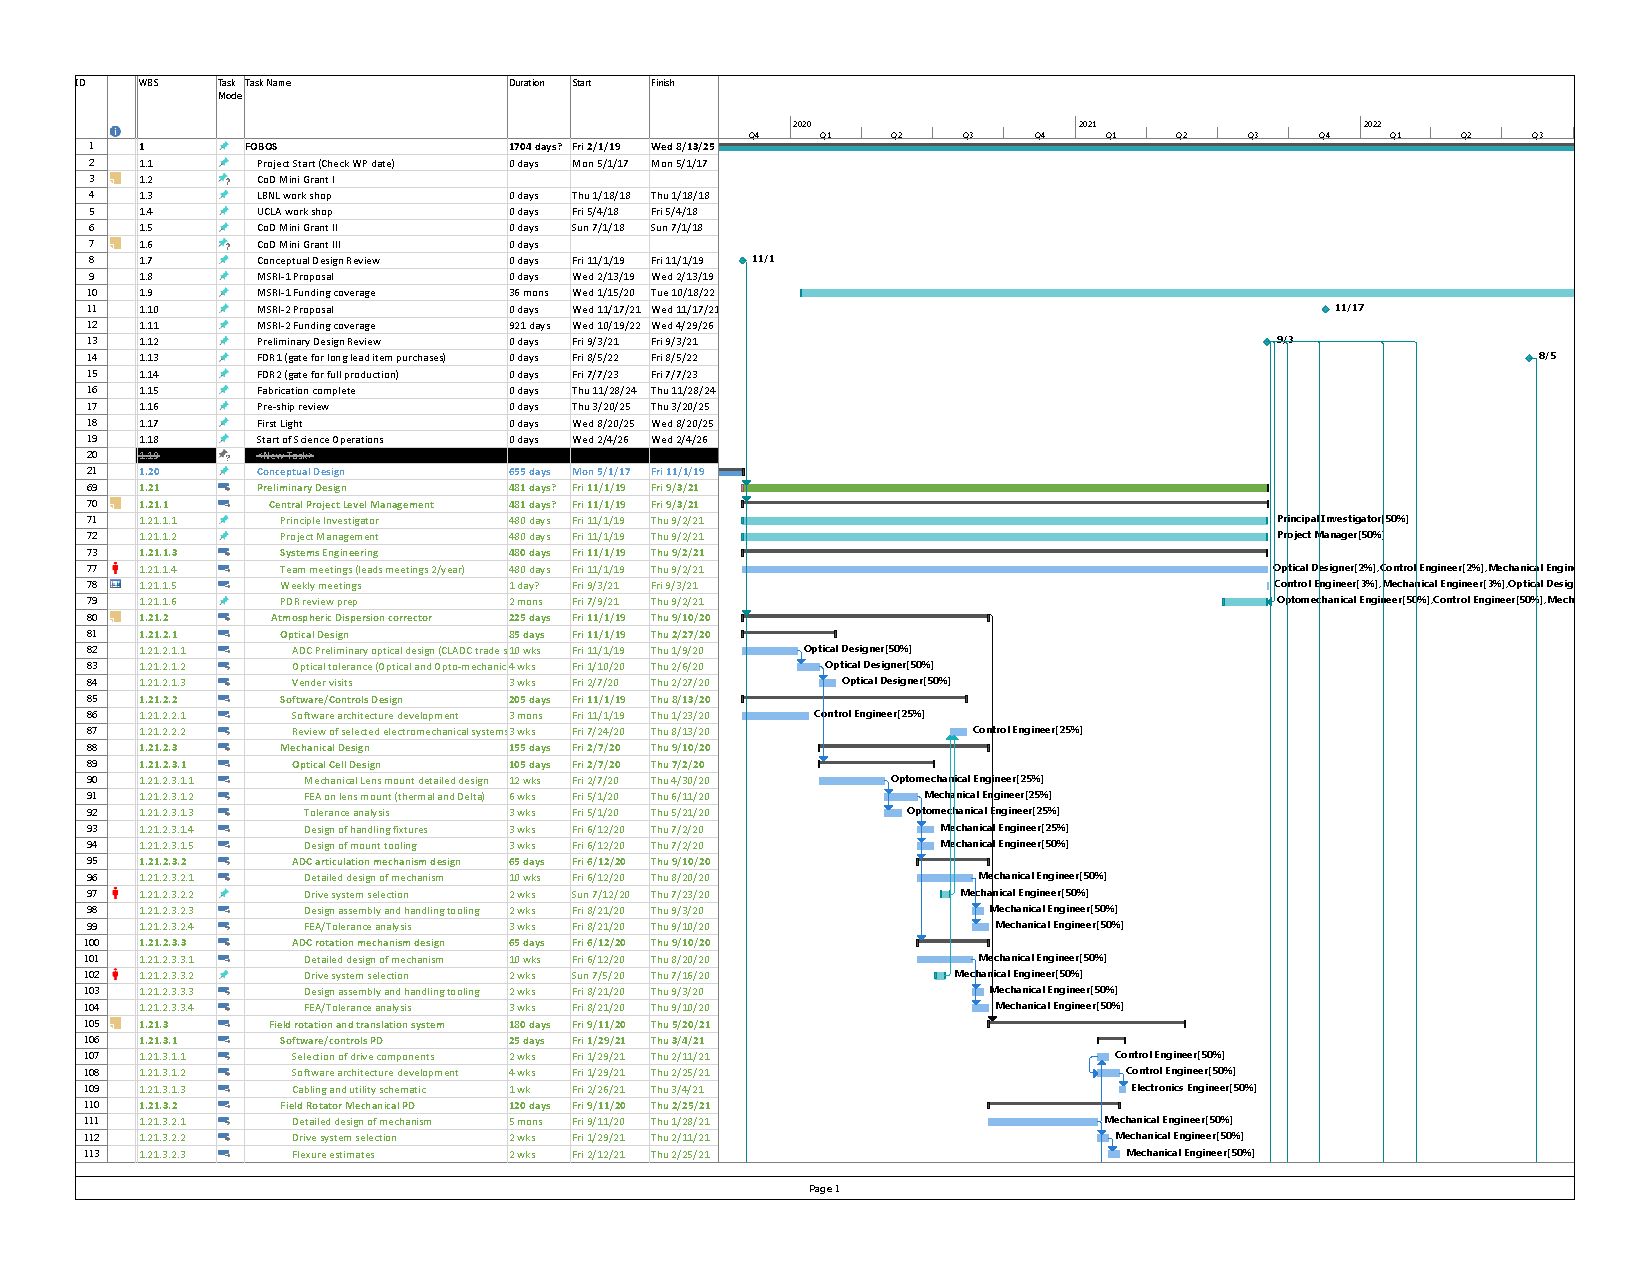
\includepdf[pages=-,landscape=true]{FOBOS_HighLevel_Schedule_v1.pdf}

\end{document}

